\documentclass[12pt]{book}

\usepackage{tabularx}
\usepackage[table]{xcolor}
\usepackage{multirow}

\usepackage{verbatim}

\usepackage[bottom]{footmisc}

\usepackage{sidecap}
\usepackage{subcaption}
\usepackage{wrapfig}

\usepackage{graphicx}

\usepackage{xcolor}
\usepackage{color}


\usepackage[most]{tcolorbox}

\tcbset{
    frame code={}
    center title,
    left=10pt,
    right=10pt,
    top=10pt,
    bottom=10pt,
    colback=gray!5,
    colframe=gray,
    width=\dimexpr\textwidth\relax,
    enlarge left by=0mm,
    boxsep=5pt,
    arc=0pt,outer arc=0pt,
}
    

\definecolor{codepurple}{rgb}{0.58,0.8,0.82}
\definecolor{backcolour}{rgb}{0.95,0.95,0.92}

\usepackage{amsmath, amssymb}
\usepackage{mathtools}

\usepackage{verbatim}

\usepackage{tikz} 
\usetikzlibrary{shapes}
\usetikzlibrary{arrows}
\usetikzlibrary{positioning}
\usetikzlibrary{patterns}
\usetikzlibrary{calc}
\usetikzlibrary{shadings, shadows}

\usepackage{hyperref}
\hypersetup{
    colorlinks=true, %set true if you want colored links
    linktoc=all,     %set to all if you want both sections and subsections linked
    linkcolor=black,  %choose some color if you want links to stand out
}

\usepackage[margin=1.4in,footskip=.25in]{geometry}


\tikzstyle{input}=[
        draw,
        trapezium,
        trapezium left angle=60,
        trapezium right angle=120,
        inner sep=10pt,
        fill=white!25
]
\tikzstyle{output}=[
        draw,
        trapezium,
        trapezium left angle=60,
        trapezium right angle=120,
        inner sep=10pt,
        fill=white!25
]
\tikzstyle{debutfin}=[ellipse,draw,text=black,inner sep=10pt]
\tikzstyle{instruct}=[rectangle,draw,fill=white!50,inner sep=10pt]
\tikzstyle{test}=[diamond, aspect=1,thick,
draw=black,fill=white!50,text=black]
\tikzstyle{es}=[rectangle,draw,rounded corners=4pt,fill=white!25,inner sep=10pt]
%styledesflèches
\tikzstyle{suite}=[->,>=stealth,thick,rounded corners=4pt]
%placementdesnœuds

\usepackage{xepersian}
\settextfont[Scale=1]{Vazir}





\makeatletter
\pgfkeys{/pgf/.cd,
  parallelepiped offset x/.initial=2mm,
  parallelepiped offset y/.initial=2mm
}


\pgfdeclareshape{parallelepiped}
{
  \inheritsavedanchors[from=rectangle] % this is nearly a rectangle
  \inheritanchorborder[from=rectangle]
  \inheritanchor[from=rectangle]{north}
  \inheritanchor[from=rectangle]{north west}
  \inheritanchor[from=rectangle]{north east}
  \inheritanchor[from=rectangle]{center}
  \inheritanchor[from=rectangle]{west}
  \inheritanchor[from=rectangle]{east}
  \inheritanchor[from=rectangle]{mid}
  \inheritanchor[from=rectangle]{mid west}
  \inheritanchor[from=rectangle]{mid east}
  \inheritanchor[from=rectangle]{base}
  \inheritanchor[from=rectangle]{base west}
  \inheritanchor[from=rectangle]{base east}
  \inheritanchor[from=rectangle]{south}
  \inheritanchor[from=rectangle]{south west}
  \inheritanchor[from=rectangle]{south east}
  \backgroundpath{
    % store lower right in xa/ya and upper right in xb/yb
    \southwest \pgf@xa=\pgf@x \pgf@ya=\pgf@y
    \northeast \pgf@xb=\pgf@x \pgf@yb=\pgf@y
    \pgfmathsetlength\pgfutil@tempdima{\pgfkeysvalueof{/pgf/parallelepiped
      offset x}}
    \pgfmathsetlength\pgfutil@tempdimb{\pgfkeysvalueof{/pgf/parallelepiped
      offset y}}
    \def\ppd@offset{\pgfpoint{\pgfutil@tempdima}{\pgfutil@tempdimb}}
    \pgfpathmoveto{\pgfqpoint{\pgf@xa}{\pgf@ya}}
    \pgfpathlineto{\pgfqpoint{\pgf@xb}{\pgf@ya}}
    \pgfpathlineto{\pgfqpoint{\pgf@xb}{\pgf@yb}}
    \pgfpathlineto{\pgfqpoint{\pgf@xa}{\pgf@yb}}
    \pgfpathclose
    \pgfpathmoveto{\pgfqpoint{\pgf@xb}{\pgf@ya}}
    \pgfpathlineto{\pgfpointadd{\pgfpoint{\pgf@xb}{\pgf@ya}}{\ppd@offset}}
    \pgfpathlineto{\pgfpointadd{\pgfpoint{\pgf@xb}{\pgf@yb}}{\ppd@offset}}
    \pgfpathlineto{\pgfpointadd{\pgfpoint{\pgf@xa}{\pgf@yb}}{\ppd@offset}}
    \pgfpathlineto{\pgfqpoint{\pgf@xa}{\pgf@yb}}
    \pgfpathmoveto{\pgfqpoint{\pgf@xb}{\pgf@yb}}
    \pgfpathlineto{\pgfpointadd{\pgfpoint{\pgf@xb}{\pgf@yb}}{\ppd@offset}}
  }
}
\makeatother



\tikzstyle{pc1}   = [
parallelepiped, 
minimum width=12pt, 
text width=12pt, 
inner sep=12pt, 
draw, 
line width=2pt, 
path picture=
	{
	\draw (-1,-1) -- ++(1,-2);
	}
]




\tikzset{
  ports/.style={
    line width=0.3pt,
    top color=gray!20,
    bottom color=gray!20
  },
  rack switch/.style={
    parallelepiped,fill=white, draw,
    minimum width=1.25cm,
    minimum height=0.25cm,
    parallelepiped offset x=2mm,
    parallelepiped offset y=1.25mm,
    xscale=-1,
    path picture={
      \draw[top color=gray!5,bottom color=gray!40]
      (path picture bounding box.south west) rectangle 
      (path picture bounding box.north east);
      \coordinate (A-west) at ([xshift=-0.2cm]path picture bounding box.west);
      \coordinate (A-center) at ($(path picture bounding box.center)!0!(path
        picture bounding box.south)$);
      \foreach \x in {0.275,0.525,0.775}{
        \draw[ports]([yshift=-0.05cm]$(A-west)!\x!(A-center)$)
          rectangle +(0.1,0.05);
        \draw[ports]([yshift=-0.125cm]$(A-west)!\x!(A-center)$)
          rectangle +(0.1,0.05);
       } 
      \coordinate (A-east) at (path picture bounding box.east);
      \foreach \x in {0.085,0.21,0.335,0.455,0.635,0.755,0.875,1}{
        \draw[ports]([yshift=-0.1125cm]$(A-east)!\x!(A-center)$)
          rectangle +(0.05,0.1);       
      }
    }
  },
  server/.style={
    parallelepiped,
    fill=white, draw,
    minimum width=0.35cm,
    minimum height=0.75cm,
    parallelepiped offset x=3mm,
    parallelepiped offset y=3mm,
    xscale=-1,
    path picture={
      \draw[top color=gray!5,bottom color=gray!40]
      (path picture bounding box.south west) rectangle 
      (path picture bounding box.north east);
      \coordinate (A-center) at ($(path picture bounding box.center)!0!(path
        picture bounding box.south)$);
      \coordinate (A-west) at ([xshift=-0.575cm]path picture bounding box.west);
      \draw[ports]([yshift=0.1cm]$(A-west)!0!(A-center)$)
        rectangle +(0.2,0.065);
      \draw[ports]([yshift=0.01cm]$(A-west)!0.085!(A-center)$)
        rectangle +(0.15,0.05);
      \fill[black]([yshift=-0.35cm]$(A-west)!-0.1!(A-center)$)
        rectangle +(0.235,0.0175);
      \fill[black]([yshift=-0.385cm]$(A-west)!-0.1!(A-center)$)
        rectangle +(0.235,0.0175);
      \fill[black]([yshift=-0.42cm]$(A-west)!-0.1!(A-center)$)
        rectangle +(0.235,0.0175);
    }  
  }
}



% Styles for interfaces and edge labels
\tikzset{%
  interface/.style={draw, rectangle, rounded corners, font=\LARGE\sffamily},
  ethernet/.style={interface, fill=yellow!50},% ethernet interface
  serial/.style={interface, fill=green!70},% serial interface
  speed/.style={sloped, anchor=south, font=\large\sffamily},% line speed at edge
  route/.style={draw, shape=single arrow, single arrow head extend=4mm,
    minimum height=1.7cm, minimum width=3mm, white, fill=white!20,
    drop shadow={opacity=.8, fill=white!50!black}, font=\tiny}% inroute / outroute arrows
}
\newcommand*{\shift}{1.3cm}% For placing the arrows later






\newcommand*{\laptop}{

\begin{tikzpicture}    
%backmonitor
\draw[thick, fill=gray!70] (0,0) rectangle (2,1.4);

%screen
\draw[thick, fill=blue!10] (0.1,0.1) rectangle (1.9,1.3);

%keyboard
\draw[thick, fill=gray!70] (0,0) -- (.5,-.7) -- (2.5,-.7) -- (2,0);
\draw[thick, fill=gray!70] (0,0) -- (0,-.1) -- (.5,-0.8) -- (2.5,-.8) -- (2.5,-.7) -- (.5,-0.7) -- (0,0);
\foreach \x in {.4,.6,.8,1,1.2,1.4,1.6,1.8,2} {
\draw (\x,-.22) -- (\x+.2,-.5);
}
\draw (.14,-.12-.1) -- (2+.14,-.12-.1);
\draw (.2,-.2-.1) -- (2+.2,-.2-.1);
\draw (.3,-.3-.1) -- (2+.3,-.3-.1);
\draw (.37,-.4-.1) -- (2+.37,-.4-.1);
%\foreach \x in {.12,.2,.3,.4} {
%\draw (\x,-\x-.1) -- (2+\x,-\x-.1);
%}
\end{tikzpicture}
}




\newcommand*{\computer}{
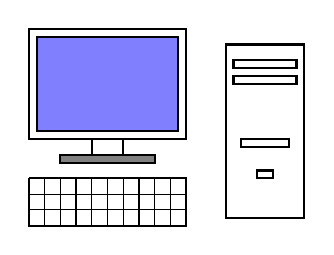
\begin{tikzpicture}   
%back monitor 
\draw[thick] (0,0) rectangle (2,1.4);
%\draw[thick] (0,1.4) -- (.1,1.5) -- (2.1,1.5) -- (2,1.4);
%\draw[thick] (2.1,1.5) -- (2.1,.1) -- (2,0);

%screen
\draw[thick, fill=blue!50] (0.1,0.1) rectangle (1.9,1.3);


%monitor LEG
\draw[thick] (.8,0) rectangle (1.2,-.2);
\draw[thick, fill=gray] (.4,-.2) rectangle (1.6,-.3);

%keyboard
\draw[thick] (0,-0.5) -- (0,-1.1) -- (2,-1.1) -- (2,-0.5) --(0,-0.5);
\foreach \x in {.2,.4,.6,.8,1,1.2,1.4,1.6,1.8} {
\draw (\x,-0.5) -- (\x,-1.1);
}
\foreach \x in {-.5,.-.7,-.9} {
\draw (0,\x) -- (2,\x);
}

%case
\draw[thick] (2.5,-1) rectangle (3.5,1.2);
\draw[thick] (2.6,.7) rectangle (3.4,.8);
\draw[thick] (2.6,.9) rectangle (3.4,1);
\draw[thick] (2.7,-.1) rectangle (3.3,0);
\draw[thick] (2.9,-.5) rectangle (3.1,-.4);

\end{tikzpicture}
}











\newcommand*{\computertwo}{
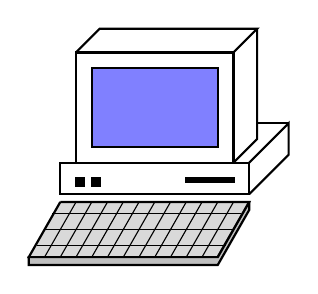
\begin{tikzpicture}   
%back monitor 
\draw[thick] (0,0) rectangle (2,1.4);
\draw[thick] (0,1.4) -- (.3,1.7) -- (2.3,1.7) -- (2,1.4);
\draw[thick] (2.3,1.7) -- (2.3,.3) -- (2,0);

%screen
\draw[thick, fill=blue!50] (0.2,0.2) rectangle (1.8,1.2);


%monitor LEG
\draw[thick] (-.2,0) rectangle (2.2,-.4);
\draw[thick] (2.2,0) -- (2.7,.5) -- (2.7,.1) -- (2.2,-.4) ;
\draw[thick] (2.7,.5) -- (2.3,.5);
%\draw[thick, fill=gray] (.4,-.2) rectangle (1.6,-.3);


%keyboard
\draw[thick, fill=gray!30] (-0.2,-.5) -- (2.2,-.5) -- (1.8,-1.2) -- (-.6,-1.2) -- (-0.2,-.5) ;
\draw[thick, fill=gray!50] (2.2,-.5) -- (2.2,-.6) -- (1.8,-1.3) --  (-.6,-1.3) -- (-.6,-1.2) -- (1.8,-1.2) -- (2.2,-.5) ;

%\draw (0,-.7) rectangle (.1,-.8);
\foreach \x in {0,.2,.4,.6,.8,1,1.2,1.4,1.6,1.8,2} {
\draw (\x,-0.5) -- (\x-.4,-1.2);
}
\draw (-0.3,-.65) -- (2.1,-.65);
\draw (-0.4,-.85) -- (2,-.85);
\draw (-0.5,-1.05) -- (1.9,-1.05);
%\foreach \x in {-.7,-.9,-1.1} {
%\draw (-0.3,\x) -- (2+0.2,\x);
%}


\draw[thick, fill=black] (0,-.2) rectangle (0.1,-.3);
\draw[thick, fill=black] (0.2,-.2) rectangle (0.3,-.3);

\draw[thick, fill=black] (1.4,-.2) rectangle (2,-.25);

\end{tikzpicture}
}















\newcommand*{\computerthree}{

\begin{tikzpicture}   
%back monitor 
\draw[thick] (0,0) rectangle (2,1.4);
%\draw[thick] (0,1.4) -- (.3,1.7) -- (2.3,1.7) -- (2,1.4);
%\draw[thick] (2.3,1.7) -- (2.3,.3) -- (2,0);

%screen
\draw[thick, fill=blue!50] (0.2,0.2) rectangle (1.8,1.2);


%monitor LEG
\draw[thick] (-.2,0) rectangle (2.2,-.4);
%\draw[thick] (2.2,0) -- (2.7,.5) -- (2.7,.1) -- (2.2,-.4) ;
%\draw[thick] (2.7,.5) -- (2.3,.5);
%\draw[thick, fill=gray] (.4,-.2) rectangle (1.6,-.3);


%keyboard
\draw[thick, fill=gray!30] (-0.2,-.5) -- (2.2,-.5) -- (2.2,-1.1) -- (-0.2,-1.1) -- (-0.2,-.5) ;
%\draw[thick, fill=gray!50] (2.2,-.5) -- (2.2,-.6) -- (1.8,-1.3) --  (-.6,-1.3) -- (-.6,-1.2) -- (1.8,-1.2) -- (2.2,-.5) ;

%\draw (0,-.7) rectangle (.1,-.8);
\foreach \x in {0,.2,.4,.6,.8,1,1.2,1.4,1.6,1.8,2} {
\draw (\x,-0.5) -- (\x,-1.1);
}
\draw (-0.2,-.7) -- (2.2,-.7);
\draw (-0.2,-.9) -- (2.2,-.9);
\draw (-0.2,-1.1) -- (2.2,-1.1);
%\foreach \x in {-.7,-.9,-1.1} {
%\draw (-0.3,\x) -- (2+0.2,\x);
%}


\draw[thick, fill=black] (0,-.2) rectangle (0.1,-.3);
\draw[thick, fill=black] (0.2,-.2) rectangle (0.3,-.3);
\draw[thick, fill=black] (1.4,-.2) rectangle (2,-.25);

\end{tikzpicture}
}









% The router icon
\newcommand*{\router}[1]{
\begin{tikzpicture}[xscale=.4,yscale=.6] 
  \coordinate (ll) at (-3,0.5);
  \coordinate (lr) at (3,0.5);
  \coordinate (ul) at (-3,2);
  \coordinate (ur) at (3,2);
  \shade [shading angle=90, left color=black!40!white, right color=white] ($(ll)+(0,.5)$) arc (-180:-60:3cm and .75cm) -- +(0,1) arc (-60:-180:3cm and .75cm)
    -- cycle;
  \shade [shading angle=270, right color=black!40!white, left color=white!50] ($(lr)+(0,.5)$) arc (0:-60:3cm and .75cm) -- +(0,1) arc (-60:0:3cm and .75cm) -- cycle;
  \draw [thick] ($(ll)+(0,.5)$) arc (-180:0:3cm and .75cm) -- (ur) arc (0:-180:3cm and .75cm)
    -- cycle;
  \draw [thick, shade, upper left=white!30!black, lower left=white!80!white, upper right=white!80!white, lower right=white] (ul) arc (-180:180:3cm and .75cm);
  \node at (0,0.5){\color{blue!60!black}\Huge #1};% The name of the router
  % The four arrows, symbols for incoming and outgoing routes:
  \begin{scope}[yshift=2cm, yscale=0.28, transform shape]
    \node[route, rotate=45, xshift=\shift] {\strut};
    \node[route, rotate=-45, xshift=-\shift] {\strut};
    \node[route, rotate=-135, xshift=\shift] {\strut};
    \node[route, rotate=135, xshift=-\shift] {\strut};
  \end{scope}
\end{tikzpicture}}




\renewcommand{\baselinestretch}{1.3} 

\begin{document}

\tableofcontents

\newpage

\chapter{مبانی کامپیوتر}

\section{الگوریتم چیست؟}

الگوریتم مجموعه ای از مرحله های محاسباتی پشت سر هم است که مقادیر ورودی را دریافت می کنند و به خروجی تبدیل می کنند

\subsection{ویژگی های الگوریتم}

\begin{enumerate}
	\item تعداد دستورالعمل ها باید مشخص باشد
	\item ابتدا و انتهای الگوریتم مشخص باشد
	\item دستورالعمل ها بدون ابهام باشند
	\item دستورالعمل ها قابل اجرا باشند
	\item الگوریتم هدف مشخصی داشته باشد
\end{enumerate}

\section{فلوچارت چیست ؟}

برای درک بهتر الگوریتم و سهولت در دنبال کردن دستورالعمل های آن از یکسری اشکال خاص برای نشان دادن الگوریتم استفاده می کنیم که به آن فلوچارت گفته می شود .

به عبارت ساده تر :

به مجموعه ای از علائم ساده که الگوریتم را به صورت نماد های تصویری یا نموداری تبدیل می کند ، فلوچارت گفته می شود .

\subsection{نماد های قراردادی در فلوچارت}

\subsubsection{ علامت شروع و پایان ، بیضی می باشد}

برای نشان دادن شروع و پایان الگوریتم استفاده می شوند .

\begin{center}
\begin{tikzpicture}
\node[debutfin] (debut) at (0,0) {شروع};
\node[debutfin] (fin) at (5,0) {پایان};
\end{tikzpicture}
\end{center}

\subsubsection{ علامت محاسبات و مقداردهی  ، مستطیل می باشد  }

برای انجام محسابات ریاضی و مقدار دهی به متغیر ها استفاده می شود

\begin{center}
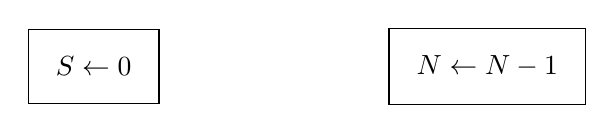
\begin{tikzpicture}
\node[instruct] (init) at (0,0) {$S\leftarrow 0$};
\node[instruct] (moins) at (5,0) {$N\leftarrow N-1$};
\end{tikzpicture}
\end{center}

\subsubsection{  
 علامت ورودی گرفتن و چاپ در خروجی ، متوازی الاضلاع می باشد }

\begin{center}
\begin{tikzpicture}
\node[input] (lire) at (0,0) { بخوان را $X$ };
\node[output] (afficher) at (5,0) { کن چاپ را $X$ };
\end{tikzpicture}
\end{center}

\subsubsection{ علامت بررسی شرط ، لوزی می باشد}

\begin{center}
\begin{tikzpicture}
\node[test] (test) at (0,0) {$N>0$};
\draw[suite] (test) -- ($(test)+(2,0)$) node[near start,yshift=7pt]{بله};
\draw[suite] (test) -- ($(test)+(-2,0)$) node[near start,yshift=7pt]{خیر};
\end{tikzpicture}
\end{center}


\newpage
\subsection{مثالهایی از الگوریتم و فلوچارت}

\subsubsection{مثال}

فلوچارتی رسم کنید که دو عدد A و B را به عنوان ورودی گرفته و حاصل جمع آنها را چاپ کند .



\begin{center}
\begin{tikzpicture}
\node[debutfin] (debut) at (0,0) {شروع};
\node[input] (lire) at (0,-2) { بخوان را $B$ و $A$ };
\node[instruct] (init) at (0,-4) {$C \leftarrow A + B$};
\node[output] (afficher) at (0,-6) { کن چاپ را $C$ };
\node[debutfin] (fin) at (0,-8) {پایان};
%Placementdesflèches
\draw[suite] (debut) -- (lire);
\draw[suite] (lire) -- (init);
\draw[suite] (init) -- (afficher);
\draw[suite] (afficher) -- (fin);
\begin{scope} [xshift=4cm,yshift=-4cm]
\draw node [right,text width=6cm,rounded corners,fill=gray!10,inner sep=1ex]
{
\begin{enumerate}
	\item [.1] شروع
	\item [.2] بخوان را
	\lr{A}
	و
	\lr{B}
	\item [.3] $C \leftarrow A + B$
	\item [.4] کن چاپ را
	\lr{C}
	\item [.5] پایان
\end{enumerate}
};
\end{scope}
\end{tikzpicture}
\end{center}


\newpage
\subsubsection{مثال}

فلوچارتی رسم کنید که دو عدد را خوانده و حاصلضرب آنها را نمایش دهد 



\begin{center}
\begin{tikzpicture}
\node[debutfin] (debut) at (0,0) {شروع};
\node[input] (lire) at (0,-2) { بخوان را $B$ و $A$ };
\node[instruct] (init) at (0,-4) {$C \leftarrow A \times B$};
\node[output] (afficher) at (0,-6) { کن چاپ را $C$ };
\node[debutfin] (fin) at (0,-8) {پایان};
%Placementdesflèches
\draw[suite] (debut) -- (lire);
\draw[suite] (lire) -- (init);
\draw[suite] (init) -- (afficher);
\draw[suite] (afficher) -- (fin);
\begin{scope} [xshift=4cm,yshift=-4cm]
\draw node [right,text width=6cm,rounded corners,fill=gray!10,inner sep=1ex]
{
\begin{enumerate}
	\item [.1] شروع
	\item [.2] بخوان را
	\lr{A}
	و
	\lr{B}
	\item [.3] $C \leftarrow A \times B$
	\item [.4] کن چاپ را
	\lr{C}
	\item [.5] پایان
\end{enumerate}
};
\end{scope}
\end{tikzpicture}
\end{center}



\newpage
\subsubsection{مثال}

فلوچارتی رسم کنید که شعاع یک دایره را خوانده و مساحت و محیط آن را نمایش دهد .



\begin{center}
\begin{tikzpicture}
\node[debutfin] (debut) at (0,0) {شروع};
\node[input] (lire) at (0,-2) { بخوان را $r$ };
\node[instruct] (init) at (0,-4) {$A \leftarrow \pi \times r \times r$};
\node[instruct] (init2) at (0,-6) {$P \leftarrow 2 \times \pi \times r $};
\node[output] (afficher) at (0,-8) { کن چاپ را $A$ و $P$ };
\node[debutfin] (fin) at (0,-10) {پایان};
%Placementdesflèches
\draw[suite] (debut) -- (lire);
\draw[suite] (lire) -- (init);
\draw[suite] (init) -- (init2);
\draw[suite] (init2) -- (afficher);
\draw[suite] (afficher) -- (fin);
\begin{scope} [xshift=4cm,yshift=-4cm]
\draw node [right,text width=6cm,rounded corners,fill=gray!10,inner sep=1ex]
{
\begin{enumerate}
	\item [.1] شروع
	\item [.2] بخوان را
	\lr{r}
	\item [.3] $A \leftarrow \pi \times r \times r$
	\item [.4] $P \leftarrow 2 \times \pi \times r$
	\item [.5] کن چاپ را
	\lr{A}
	و
	\lr{P}
	\item [.6] پایان
\end{enumerate}
};
\end{scope}
\end{tikzpicture}
\end{center}


\newpage
\subsubsection{مثال}

فلوچارتی رسم کنید که دو عدد را خوانده و سپس مقادیر آن دو عدد را با هم جا به جا کند .



\begin{center}
\begin{tikzpicture}
\node[debutfin] (a) at (0,0) {شروع};
\node[input] (b) at (0,-2) { بخوان را $B$ و $A$ };
\node[instruct] (c) at (0,-4) {$T \leftarrow A$};
\node[instruct] (d) at (0,-6) {$A \leftarrow B$};
\node[instruct] (e) at (0,-8) {$B \leftarrow T$};
\node[output] (f) at (0,-10) { کن چاپ را $A$ و $B$ };
\node[debutfin] (g) at (0,-12) {پایان};
%Placementdesflèches
\draw[suite] (a) -- (b);
\draw[suite] (b) -- (c);
\draw[suite] (c) -- (d);
\draw[suite] (d) -- (e);
\draw[suite] (e) -- (f);
\draw[suite] (f) -- (g);
\begin{scope} [xshift=4cm,yshift=-4cm]
\draw node [right,text width=6cm,rounded corners,fill=gray!10,inner sep=1ex]
{
\begin{enumerate}
	\item [.1]  شروع
	\item [.2]  بخوان را
	\lr{B}
	و
	\lr{A}

	\item [.3]  $T \leftarrow A$
	\item [.4]  $A \leftarrow B$
	\item [.5] $B \leftarrow T$
	\item [.6] کن چاپ را
	 \lr{B}
	و
	\lr{A}
	\item [.7]  پایان
\end{enumerate}
};
\end{scope}
\end{tikzpicture}
\end{center}


\newpage
\subsubsection{مثال}

فلوچارتی رسم کنید که یک عدد را دریافت کند و مشخص کند که عدد زوج است یا فرد 

\begin{itemize}
	\item یک عدد زوج است وقتی باقی مانده ی تقسیم آن عدد بر 2 برابر صفر باشد
	\item یک عدد فرد است وقتی باقی مانده ی تقسیم آن عدد بر 2 برابر با صفر نباشد
\end{itemize}

\begin{center}
\begin{tikzpicture}
\node[debutfin] (a) at (0,0) {شروع};
\node[input] (b) at (0,-2) { بخوان را $X$ };
\node[instruct] (c) at (0,-4) {$D \leftarrow X / 2$};
\node[instruct] (d) at (0,-6) {$R \leftarrow X - 2 \times D$};
\node[test] (test) at (0,-8) {$R = 0$};
\node[output] (e) at (2,-10) {است زوج $X$};
\node[output] (f) at (-2,-10) {است فرد $X$};
\node[debutfin] (g) at (0,-13) {پایان};
%Placementdesflèches
\draw[suite] (a) -- (b);
\draw[suite] (b) -- (c);
\draw[suite] (c) -- (d);
\draw[suite] (d) -- (test);
\draw[suite] (test) -| (e) node[near start,yshift=7pt]{بله};
\draw[suite] (test) -| (f) node[near start,yshift=7pt]{خیر};
\draw[suite] (e) |- (0,-11.5) -- (g);
\draw[suite] (f) |- (0,-11.5) -- (g);
\begin{scope} [xshift=4.5cm,yshift=-5cm]
\draw node [right,text width=6cm,rounded corners,fill=gray!10,inner sep=1ex]
{
\begin{enumerate}
	\item [.1]  شروع
	\item [.2]  بخوان را
	\lr{X}
	\item [.3]  $D \leftarrow X / 2$
	\item [.4]  $R \leftarrow X - 2 \times D$
	\item [.5]  \lr{if (R $=$ 0) goto $\to$ 6 \qquad else goto $\to$ 7}
	\item [.6] کن چاپ را
	است زوج
	 \lr{X}
	 \lr{\qquad goto $\to$ 8}
	\item [.7] کن چاپ را
	است فرد
	 \lr{X}
	 \lr{\qquad goto $\to$ 8}
	\item [.8]  پایان
\end{enumerate}
};
\end{scope}
\end{tikzpicture}
\end{center}



\newpage
\subsubsection{مثال}


فلوچارتی رسم کنید که عملکرد قدر مطلق را انجام دهد 

$$
|x| = \begin{cases}
x \geq 0 \qquad x \\
x < 0 \qquad -x 
\end{cases}
$$


\begin{center}
\begin{tikzpicture}
\node[debutfin] (a) at (0,0) {شروع};
\node[input] (b) at (0,-2) { بخوان را $X$ };
\node[test] (test) at (0,-4) {$X \geq 0$};
\node[instruct] (e) at (-2,-6) {$X \leftarrow -1 \times X$};
\node[output] (f) at (0,-9) { کن چاپ را $X$ };
\node[debutfin] (g) at (0,-11) {پایان};
%Placementdesflèches
\draw[suite] (a) -- (b);
\draw[suite] (b) -- (test);
\draw[suite] (test) -| (2,-6) node[near start,yshift=7pt]{بله} |- (0,-7.5) -- (f);
\draw[suite] (test) -| (e) node[near start,yshift=7pt]{خیر};
%\draw[suite] (d) |- (0,-7.5) -- (f);
\draw[suite] (e) |- (0,-7.5) -- (f);
\draw[suite] (f) -- (g);
\begin{scope} [xshift=4cm,yshift=-4cm]
\draw node [right,text width=6cm,rounded corners,fill=gray!10,inner sep=1ex]
{
\begin{enumerate}
	\item [.1]  شروع
	\item [.2]  بخوان را
	\lr{X}
	\item [.3]  \lr{if (X $\geq$ 0) goto $\to$ 5 \qquad else goto $\to$ 4}
	\item [.4] $X \leftarrow -1 \times X$
	\item [.5] کن چاپ را
	\lr{X}
	\item [.6]  پایان
\end{enumerate}
};
\end{scope}
\end{tikzpicture}
\end{center}



\newpage
\subsubsection{مثال}

فلوچارتی رسم کنید که عدد X را از ورودی بخواند و 
\begin{itemize}
	\item اگر X مثبت بود ، آن را در 2 ضرب کند و چاپ نماید
	\item اگر X منفی بود قدر مطلق X را چاپ کند 
\end{itemize}


\begin{center}
\begin{tikzpicture}
\node[debutfin] (a) at (0,0) {شروع};
\node[input] (b) at (0,-2) { بخوان را $X$ };
\node[test] (test) at (0,-4) {$X \geq 0$};
\node[instruct] (d) at (2,-6) {$X \leftarrow 2 \times X$};
\node[instruct] (e) at (-2,-6) {$X \leftarrow -1 \times X$};
\node[output] (f) at (0,-9) { کن چاپ را $X$ };
\node[debutfin] (g) at (0,-11) {پایان};
%Placementdesflèches
\draw[suite] (a) -- (b);
\draw[suite] (b) -- (test);
\draw[suite] (test) -| (d) node[near start,yshift=7pt]{بله};
\draw[suite] (test) -| (e) node[near start,yshift=7pt]{خیر};
\draw[suite] (d) |- (0,-7.5) -- (f);
\draw[suite] (e) |- (0,-7.5) -- (f);
\draw[suite] (f) -- (g);
\begin{scope} [xshift=4cm,yshift=-4.5cm]
\draw node [right,text width=6cm,rounded corners,fill=gray!10,inner sep=1ex]
{
\begin{enumerate}
	\item [.1]  شروع
	\item [.2]  بخوان را
	\lr{X}
	\item [.3]  \lr{if (X $\geq$ 0) goto $\to$ 5 \qquad else goto $\to$ 4}
	\item [.4] $X \leftarrow -1 \times X$
	\lr{\qquad\qquad goto $\to$ 6}
	\item [.5] $X \leftarrow 2 \times X$
	\lr{\qquad\qquad\qquad goto $\to$ 6}
	\item [.6] کن چاپ را
	\lr{X}
	\item [.7]  پایان
\end{enumerate}
};
\end{scope}
\end{tikzpicture}
\end{center}


\newpage
\subsubsection{مثال}

فلوچارتی رسم کنید که عدد N را دریافت کند و N جمله ی اول دنباله ی 
$$
1 , 2 , 4 , 7 , 11 , 16 , \dots
$$

را چاپ کند 


\begin{center}
\begin{tikzpicture}
\node[debutfin] (a) at (0,0) {شروع};
\node[instruct] (b) at (0,-2) {$S \leftarrow 1 , C \leftarrow 1$};
\node[input] (c) at (0,-3.6) {بخوان را $N$};
\node[test] (test) at (0,-6) {$N > 0$};
\node[output] (d) at (3,-8) {کن چاپ را $S$};
\node[instruct] (f) at (3,-10) {$S \leftarrow S + C$};
\node[instruct] (g) at (3,-12) {$C \leftarrow C + 1$};
\node[instruct] (h) at (3,-14) {$N \leftarrow N - 1$};
\node[debutfin] (i) at (-3,-10) {پایان};
%Placementdesflèches
\draw[suite] (a) -- (b);
\draw[suite] (b) -- (c);
\draw[suite] (c) -- (test);
\draw[suite] (test) -| (d) node[near start,yshift=7pt]{بله};
\draw[suite] (test) -| (i) node[near start,yshift=7pt]{خیر};
\draw[suite] (d) -- (f);
\draw[suite] (f) -- (g);
\draw[suite] (g) -- (h);
\draw[suite] (h) -| (test);
\begin{scope} [xshift=5.5cm,yshift=-6cm]
\draw node [right,text width=6cm,rounded corners,fill=gray!10,inner sep=1ex]
{
\begin{enumerate}
	\item [.1]  شروع
	\item [.2] $S \leftarrow 1 , C \leftarrow 1$
	\item [.3]  بخوان را
	\lr{N}
	\item [.4]  \lr{if (N $>$ 0) goto $\to$ 5 \qquad else goto $\to$ 9}
	\item [.5] کن چاپ را
	\lr{S}
	\item [.6] $S \leftarrow S + C$
	\item [.7] $C \leftarrow C + 1$
	\item [.8] $N \leftarrow N - 1$
	\lr{\qquad\qquad\qquad goto $\to$ 4}
	\item [.9]  پایان
\end{enumerate}
};
\end{scope}
\end{tikzpicture}
\end{center}


\newpage
\subsubsection{مثال}

فلوچارتی رسم کنید که عدد طبیعی N را از ورودی بخواند و مجموع و حاصل ضرب تعداد ارقام آن را محاسبه و چاپ نماید 




\begin{center}
\begin{tikzpicture}
\node[debutfin] (a) at (0,0) {شروع};
\node[instruct] (b) at (0,-2) {$S \leftarrow 0 , P \leftarrow 1$};
\node[input] (c) at (0,-4) {بخوان را $N$};
\node[test] (test) at (0,-6) {$N > 0$};
\node[instruct] (d) at (3,-8) {$D \leftarrow N / 10$};
\node[instruct] (e) at (3,-10) {$R \leftarrow N - D \times 10$};
\node[instruct] (f) at (3,-12) {$P \leftarrow P \times R$};
\node[instruct] (g) at (3,-14) {$S \leftarrow S + R$};
\node[instruct] (h) at (3,-16) {$N \leftarrow D$};
\node[output] (i) at (-3,-8) {کن چاپ را $S$};
\node[output] (j) at (-3,-10) {کن چاپ را $P$};
\node[debutfin] (k) at (-3,-12) {پایان};
%Placementdesflèches
\draw[suite] (a) -- (b);
\draw[suite] (b) -- (c);
\draw[suite] (c) -- (test);
\draw[suite] (test) -| (d) node[near start,yshift=7pt]{بله};
\draw[suite] (test) -| (i) node[near start,yshift=7pt]{خیر};
\draw[suite] (d) -- (e);
\draw[suite] (e) -- (f);
\draw[suite] (f) -- (g);
\draw[suite] (g) -- (h);
\draw[suite] (h) -| (test);
\draw[suite] (i) -- (j);
\draw[suite] (j) -- (k);
\begin{scope} [xshift=5.5cm,yshift=-6.5cm]
\draw node [right,text width=6cm,rounded corners,fill=gray!10,inner sep=1ex]
{
\begin{enumerate}
	\item [.1]  شروع
	\item [.2] $S \leftarrow 0 , P \leftarrow 1$
	\item [.3]  بخوان را
	\lr{N}
	\item [.4]  \lr{if (N $>$ 0) goto $\to$ 5 \qquad else goto $\to$ 10}
	\item [.5] $D \leftarrow N / 10$
	\item [.6] $R \leftarrow N - D \times 10$
	\item [.7] $P \leftarrow P \times R$
	\item [.8] $S \leftarrow S + R$
	\item [.9] $N \leftarrow D$
	\lr{\qquad\qquad\qquad\qquad goto $\to$ 4}
	\item [.10] کن چاپ را
	\lr{S}
	\item [.11] کن چاپ را
	\lr{P}
	\item [.12]  پایان
\end{enumerate}
};
\end{scope}
\end{tikzpicture}
\end{center}



\newpage
\subsubsection{مثال}


فلوچارتی رسم کنید که دو عدد طبیعی M و N را از ورودی بخواند و حاصل ضرب آنها را از طریق جمع های متوالی به دست آورد 



\begin{center}
\begin{tikzpicture}
\node[debutfin] (a) at (0,0) {شروع};
\node[input] (b) at (0,-2) { بخوان را $N$ و $M$ };
\node[test] (test) at (0,-4) {$N > 0$};
\node[instruct] (c) at (3,-6) {$M \leftarrow M + M$};
\node[instruct] (d) at (3,-8) {$N \leftarrow N - 1$};
\node[output] (e) at (-3,-6) { کن چاپ را $M$ };
\node[debutfin] (f) at (-3,-8) {پایان};
%Placementdesflèches
\draw[suite] (a) -- (b);
\draw[suite] (b) -- (test);
\draw[suite] (test) -| (c) node[near start,yshift=7pt]{بله};
\draw[suite] (test) -| (e) node[near start,yshift=7pt]{خیر};
\draw[suite] (c) -- (d);
\draw[suite] (d) -| (test);
\draw[suite] (e) -- (f);
\end{tikzpicture}
\end{center}


\newpage
\subsubsection{مثال}

فلوچارتی رسم کنید که عدد صحیح و مثبت N را دریافت کند و باقی مانده و خارج قسمت تقسیم آن بر 2 را از طریق تفریق های متوالی به دست آورد 

\begin{center}
\begin{tikzpicture}
\node[debutfin] (a) at (0,0) {شروع};
\node[input] (b) at (0,-2) { بخوان را $N$ };
\node[instruct] (c) at (0,-4) {$C \leftarrow 0$};
\node[test] (test) at (0,-6) {$N > 2$};
\node[instruct] (d) at (3,-8) {$N \leftarrow N - 2$};
\node[instruct] (e) at (3,-10) {$C \leftarrow C + 1$};
\node[output] (f) at (-3,-8) { کن چاپ را $C$ };
\node[output] (g) at (-3,-10) { کن چاپ را $N$ };
\node[debutfin] (h) at (-3,-12) {پایان};
%Placementdesflèches
\draw[suite] (a) -- (b);
\draw[suite] (b) -- (c);
\draw[suite] (c) -- (test);
\draw[suite] (test) -| (d) node[near start,yshift=7pt]{بله};
\draw[suite] (test) -| (f) node[near start,yshift=7pt]{خیر};
\draw[suite] (d) -- (e);
\draw[suite] (e) -| (test);
\draw[suite] (f) -- (g);
\draw[suite] (g) -- (h);
\end{tikzpicture}
\end{center}



\newpage
\subsubsection{مثال}

فلوچارتی رسم کنید که یک عدد را از ورودی بخواند و فاکتوریل آن را محاسبه کند .

فاکتوریل عدد n را با 
$n!$
نشان می دهند و برابر است با :

$$
n! = n \times (n-1) \times (n-2) \times (n-3) \times \dots \times 1 
$$

\begin{center}
\begin{tikzpicture}
\node[debutfin] (a) at (0,0) {شروع};
\node[input] (b) at (0,-2) { بخوان را $N$ };
\node[instruct] (c) at (0,-4) {$fact \leftarrow 1$};
\node[test] (test) at (0,-6) {$N \geq 1$};
\node[instruct] (d) at (3,-8) {$fact \leftarrow fact \times N$};
\node[instruct] (e) at (3,-10) {$N \leftarrow N - 1$};
\node[output] (f) at (-3,-8) { کن چاپ را $fact$ };
\node[debutfin] (g) at (-3,-10) {پایان};
%Placementdesflèches
\draw[suite] (a) -- (b);
\draw[suite] (b) -- (c);
\draw[suite] (c) -- (test);
\draw[suite] (test) -| (d) node[near start,yshift=7pt]{بله};
\draw[suite] (test) -| (f) node[near start,yshift=7pt]{خیر};
\draw[suite] (d) -- (e);
\draw[suite] (e) -| (test);
\draw[suite] (f) -- (g);
\end{tikzpicture}
\end{center}



\newpage
\subsubsection{مثال}

فلوچارتی رسم کنید که مجموع اعداد 1 تا 100 را چاپ کند .


\begin{center}
\begin{tikzpicture}
\node[debutfin] (a) at (0,0) {شروع};
\node[instruct] (b) at (0,-2) {$I \leftarrow 100$};
\node[instruct] (c) at (0,-4) {$Sum \leftarrow 0$};
\node[test] (test) at (0,-6) {$I \geq 1$};
\node[instruct] (d) at (3,-8) {$Sum \leftarrow Sum + I$};
\node[instruct] (e) at (3,-10) {$I \leftarrow I - 1$};
\node[output] (f) at (-3,-8) { کن چاپ را $Sum$ };
\node[debutfin] (g) at (-3,-10) {پایان};
%Placementdesflèches
\draw[suite] (a) -- (b);
\draw[suite] (b) -- (c);
\draw[suite] (c) -- (test);
\draw[suite] (test) -| (d) node[near start,yshift=7pt]{بله};
\draw[suite] (test) -| (f) node[near start,yshift=7pt]{خیر};
\draw[suite] (d) -- (e);
\draw[suite] (e) -| (test);
\draw[suite] (f) -- (g);
\end{tikzpicture}
\end{center}



\newpage
\subsubsection{مثال}

فلوچارتی رسم کنید که تا زمانی که ورودی بزرگتر از صفر باشد 
از ورودی اعداد را دریافت کند و در انتها مجموع اعداد را نشان دهد


\begin{center}
\begin{tikzpicture}
\node[debutfin] (a) at (0,0) {شروع};
\node[input] (b) at (0,-2) {بخوان را $X$};
\node[instruct] (c) at (0,-4) {$Sum \leftarrow 0$};
\node[test] (test) at (0,-6) {$X > 0$};
\node[instruct] (d) at (3,-8) {$Sum \leftarrow Sum + X$};
\node[input] (e) at (3,-10) {بخوان را $X$};
\node[output] (f) at (-3,-8) { کن چاپ را $Sum$ };
\node[debutfin] (g) at (-3,-10) {پایان};
%Placementdesflèches
\draw[suite] (a) -- (b);
\draw[suite] (b) -- (c);
\draw[suite] (c) -- (test);
\draw[suite] (test) -| (d) node[near start,yshift=7pt]{بله};
\draw[suite] (test) -| (f) node[near start,yshift=7pt]{خیر};
\draw[suite] (d) -- (e);
\draw[suite] (e) -| (test);
\draw[suite] (f) -- (g);
\end{tikzpicture}
\end{center}



\newpage
\subsubsection{مثال}

فلوچارتی رسم کنید که 100 عدد را دریافت کند و بزرگترین آنها را نشان دهد 



\begin{center}
\begin{tikzpicture}
\node[debutfin] (a) at (0,0) {شروع};
\node[instruct] (b) at (0,-2) {$I \leftarrow 100$};
\node[input] (c) at (0,-4) {بخوان را $X$};
\node[instruct] (d) at (0,-6) {$MAX \leftarrow X$};
\node[test] (test) at (0,-8) {$I > 1$};
\node[input] (e) at (5,-10) {بخوان را $X$};
\node[test] (test2) at (5,-13) {$X > MAX$};
\node[instruct] (h) at (7,-15) {$MAX \leftarrow X$};
\node[instruct] (f) at (2,-16) {$I \leftarrow I - 1$};
\node[output] (i) at (-5,-12) {کن چاپ را $MAX$};
\node[debutfin] (j) at (-5,-14) {پایان};
%Placementdesflèches
\draw[suite] (a) -- (b);
\draw[suite] (b) -- (c);
\draw[suite] (c) -- (d);
\draw[suite] (d) -- (test);
\draw[suite] (test) -| (e) node[near start,yshift=7pt]{بله};
\draw[suite] (test) -| (i) node[near start,yshift=7pt]{خیر};
\draw[suite] (e) -- (test2);

\draw[suite] (test2) -| (h) node[near start,yshift=7pt]{بله};
\draw[suite] (test2) -| (f) node[near start,yshift=7pt]{خیر};

\draw[suite] (h) |- (f);
\draw[suite] (f) -| (test);


\draw[suite] (i) -- (j);
\end{tikzpicture}
\end{center}



\newpage
\subsubsection{مثال}

فلوچارتی رسم کنید که سه عدد را از ورودی دریافت کند و بزرگترین آنها را چاپ کند 



\begin{center}
\begin{tikzpicture}
\node[debutfin] (a) at (0,0) {شروع};
\node[input] (b) at (0,-2) {بخوان را $A$ و $B$ و $C$};
\node[test] (test) at (0,-4) {$A > B$};
\node[test] (test2) at (4,-10) {$B > C$};
\node[test] (test3) at (-3,-6) {$A > C$};
\node[output] (f1) at (-5,-8) { کن چاپ را $A$ };
\node[output] (f2) at (-1,-8) { کن چاپ را $C$ };
\node[output] (f3) at (2,-12) { کن چاپ را $B$ };
\node[output] (f4) at (6,-12) { کن چاپ را $C$ };
\node[debutfin] (g) at (0,-16) {پایان};
%Placementdesflèches
\draw[suite] (a) -- (b);
\draw[suite] (b) -- (test);

\draw[suite] (test) -| (test2) node[near start,yshift=8pt]{خیر};
\draw[suite] (test) -| (test3) node[near start,yshift=8pt]{بله};

\draw[suite] (test2) -| (f3) node[near start,yshift=8pt]{بله};
\draw[suite] (test2) -| (f4) node[near start,yshift=8pt]{خیر};


\draw[suite] (test3) -| (f1) node[near start,yshift=8pt]{بله};
\draw[suite] (test3) -| (f2) node[near start,yshift=8pt]{خیر};

\draw[suite] (f1) |- (0,-14) -- (g);
\draw[suite] (f2) |- (0,-14) -- (g);
\draw[suite] (f3) |- (0,-14) -- (g);
\draw[suite] (f4) |- (0,-14) -- (g);

\end{tikzpicture}
\end{center}







\subsubsection{مثال}

در مثال قبل برای اینکه دستور
\begin{tikzpicture}
\node[output] (a) at (0,0) { کن چاپ را $C$ };
\end{tikzpicture}
را دوبار به کار نبریم می توانیم فلوچارت را به صورت زیر بکشیم .


\begin{tikzpicture}
\node[debutfin] (a) at (0,0) {شروع};
\node[input] (b) at (0,-2) {بخوان را $A$ و $B$ و $C$};
\node[test] (test) at (0,-4) {$A > B$};
\node[test] (test2) at (4,-10) {$B > C$};
\node[test] (test3) at (-3,-6) {$A > C$};
\node[output] (f1) at (-5,-8) { کن چاپ را $A$ };
\node[output] (f2) at (0,-10) { کن چاپ را $C$ };
%\node[output] (f3) at (2,-12) { کن چاپ را $C$ };
\node[output] (f4) at (6,-12) { کن چاپ را $B$ };
\node[debutfin] (g) at (0,-16) {پایان};
%Placementdesflèches
\draw[suite] (a) -- (b);
\draw[suite] (b) -- (test);

\draw[suite] (test) -| (test2) node[near start,yshift=8pt]{خیر};
\draw[suite] (test) -| (test3) node[near start,yshift=8pt]{بله};

\draw[suite] (test2) -- (f2) node[near start,yshift=8pt]{خیر};
\draw[suite] (test2) -| (f4) node[near start,yshift=8pt]{بله};


\draw[suite] (test3) -| (f1) node[near start,yshift=8pt]{بله};
\draw[suite] (test3) -| (f2) node[near start,yshift=8pt]{خیر};

\draw[suite] (f1) |- (0,-14) -- (g);
\draw[suite] (f2) -- (0,-14) -- (g);
%\draw[suite] (f3) |- (0,-14) -- (g);
\draw[suite] (f4) |- (0,-14) -- (g);

%\draw[suite] (0,-9) -- (g);
\end{tikzpicture}





\newpage
\subsubsection{مثال}

همچنین می توانیم مثال قبل را به صورت کلی حل کنیم و مقدار شمارنده را 3 در نظر بگیریم

\begin{center}
\begin{tikzpicture}
\node[debutfin] (a) at (0,0) {شروع};
\node[instruct] (b) at (0,-2) {$I \leftarrow 3$};
\node[input] (c) at (0,-4) {بخوان را $X$};
\node[instruct] (d) at (0,-6) {$MAX \leftarrow X$};
\node[test] (test) at (0,-8) {$I > 1$};
\node[input] (e) at (5,-10) {بخوان را $X$};
\node[test] (test2) at (5,-13) {$X > MAX$};
\node[instruct] (h) at (7,-15) {$MAX \leftarrow X$};
\node[instruct] (f) at (2,-16) {$I \leftarrow I - 1$};
\node[output] (i) at (-5,-12) {کن چاپ را $MAX$};
\node[debutfin] (j) at (-5,-14) {پایان};
%Placementdesflèches
\draw[suite] (a) -- (b);
\draw[suite] (b) -- (c);
\draw[suite] (c) -- (d);
\draw[suite] (d) -- (test);
\draw[suite] (test) -| (e) node[near start,yshift=7pt]{بله};
\draw[suite] (test) -| (i) node[near start,yshift=7pt]{خیر};
\draw[suite] (e) -- (test2);

\draw[suite] (test2) -| (h) node[near start,yshift=7pt]{بله};
\draw[suite] (test2) -| (f) node[near start,yshift=7pt]{خیر};

\draw[suite] (h) |- (f);
\draw[suite] (f) -| (test);


\draw[suite] (i) -- (j);
\end{tikzpicture}
\end{center}


\newpage
\subsubsection{مثال}

فلوچارتی رسم کنید که اعداد فرد بین 1 تا 100 را چاپ کند


\begin{center}
\begin{tikzpicture}
\node[debutfin] (a) at (0,0) {شروع};
\node[instruct] (b) at (0,-2) {$I \leftarrow 1$};
\node[test] (test) at (0,-4) {$I \leq 100$};
\node[instruct] (c) at (3,-6) {$D \leftarrow I / 2$};
\node[instruct] (d) at (3,-8) {$R \leftarrow I - D \times 2$};
\node[test] (test2) at (3,-10) {$R \neq 0$};
\node[input] (f) at (6,-12) { کن چاپ را $I$ };
\node[instruct] (g) at (3,-14) {$I \leftarrow I + 1$};
\node[debutfin] (h) at (-3,-10) {پایان};
%Placementdesflèches
\draw[suite] (a) -- (b);
\draw[suite] (b) -- (test);
\draw[suite] (test) -| (c) node[near start,yshift=7pt]{بله};
\draw[suite] (test) -| (h) node[near start,yshift=7pt]{خیر};
\draw[suite] (c) -- (d);
\draw[suite] (d) -- (test2);
\draw[suite] (test2) -| (f) node[near start,yshift=8pt]{بله};
\draw[suite] (test2) -- (g) node[near start,xshift=-10pt]{خیر};
\draw[suite] (f) |- (g);
\draw[suite] (g) -| (test);
\end{tikzpicture}
\end{center}




\newpage
\subsubsection{مثال}


فلوچارتی رسم کنید که میانگین اعداد زوج بین 1 تا 100 را چاپ کند

\begin{center}
\begin{tikzpicture}
\node[debutfin] (a) at (0,0) {شروع};
\node[instruct] (b) at (0,-2) {$I \leftarrow 1 \:,\: Sum \leftarrow 0 \:,\: C \leftarrow 0$};
\node[test] (test) at (0,-4) {$I \leq 100$};
\node[instruct] (e) at (3,-6) {$D \leftarrow I / 2$};
\node[instruct] (f) at (3,-8) {$R \leftarrow I - D \times 2$};
\node[test] (test2) at (3,-10) {$R = 0$};
\node[instruct] (g) at (7,-12) {$Sum \leftarrow Sum + I$};
\node[instruct] (m) at (7,-14) {$C \leftarrow C + 1$};
\node[instruct] (k) at (3,-14) {$I \leftarrow I + 1$};
\node[instruct] (h) at (-3,-8) {$Avg \leftarrow Sum / C$};
\node[output] (i) at (-3,-10) { کن چاپ را $Avg$ };
\node[debutfin] (j) at (-3,-12) {پایان};
%Placementdesflèches
\draw[suite] (a) -- (b);
\draw[suite] (b) -- (test);
\draw[suite] (test) -| (e) node[near start,yshift=7pt]{بله};
\draw[suite] (test) -| (h) node[near start,yshift=7pt]{خیر};
\draw[suite] (e) -- (f);
\draw[suite] (f) -- (test2) ;
\draw[suite] (test2) -| (g) node[near start,yshift=8pt]{بله};
\draw[suite] (test2) -- (k) node[near start,xshift=-10pt]{خیر};
\draw[suite] (g) -- (m);
\draw[suite] (m) -- (k);
\draw[suite] (k) -| (test);
\draw[suite] (test) -| (h);
\draw[suite] (h) -- (i);
\draw[suite] (i) -- (j);
\end{tikzpicture}
\end{center}



\newpage
\subsubsection{مثال}

تبدیل از مبنای 2 به مبنای 10


\begin{center}
\begin{tikzpicture}
\node[debutfin] (a) at (0,0) {شروع};
\node[instruct] (b) at (0,-1.8) {$M \leftarrow 1 \:,\: S \leftarrow 0 \:,\: C \leftarrow 0$};
\node[input] (c) at (0,-3.5) {بخوان را $X$};
\node[test] (test) at (0,-5.5) {$X > 0$};
\node[instruct] (d) at (4,-8) {$D \leftarrow X / 10$};
\node[instruct] (e) at (4,-10) {$R \leftarrow X - 10 \times D$};
\node[instruct] (f) at (4,-12) {$I \leftarrow C$};
\node[test] (test3) at (4,-14) {$I > 0$};
\node[instruct] (g) at (7,-15) {$M \leftarrow 2 \times M$};
\node[instruct] (h) at (7,-16.5) {$I \leftarrow I - 1$};
\node[instruct] (ii) at (0,-8) {$X \leftarrow D$};
\node[instruct] (i) at (0,-9.5) {$M \leftarrow 1$};
\node[instruct] (j) at (0,-11) {$C \leftarrow C + 1$};
\node[instruct] (k) at (0,-12.5) {$S \leftarrow S + M$};
\node[instruct] (l) at (0,-14) {$M \leftarrow R \times M$};
\node[output] (m) at (-4,-8) {کن چاپ را $S$};
\node[debutfin] (n) at (-4,-11) {پایان};
%Drawing Edges
\draw[suite] (a) -- (b);
\draw[suite] (b) -- (c);
\draw[suite] (c) -- (test);
\draw[suite] (test) -| (d) node[near start,yshift=7pt]{بله};
\draw[suite] (test) -| (m) node[near start,yshift=7pt]{خیر};
\draw[suite] (d) -- (e);
\draw[suite] (e) -- (f) ;
\draw[suite] (f) -- (test3);
\draw[suite] (test3) -| (g) node[near start,yshift=8pt]{بله};
\draw[suite] (test3) -- (l) node[near start,yshift=-10pt]{خیر};
\draw[suite] (g) -- (h);
\draw[suite] (h) -| (test3);
\draw[suite] (l) -- (k);
\draw[suite] (k) -- (j);
\draw[suite] (j) -- (i);
\draw[suite] (i) -- (ii);
\draw[suite] (ii) -- (test);
\draw[suite] (m) -- (n);
\end{tikzpicture}
\end{center}




\newpage
\subsubsection{مثال}

تبدیل از مبنای 2 به مبنای 10 ، به روشی بهینه تر ( چرا ؟ )


\begin{center}
\begin{tikzpicture}
\node[debutfin] (a) at (0,0) {شروع};
\node[instruct] (b) at (0,-1.8) {$M \leftarrow 1 \:,\: S \leftarrow 0 \:,\: C \leftarrow 0$};
\node[input] (c) at (0,-3.5) {بخوان را $X$};
\node[test] (test) at (0,-5.5) {$X > 0$};
\node[instruct] (d) at (4,-6.5) {$D \leftarrow X / 10$};
\node[instruct] (e) at (4,-8) {$R \leftarrow X - 10 \times D$};
\node[test] (test2) at (4,-10) {$R \neq 0$};
\node[instruct] (f) at (6,-12) {$I \leftarrow C$};
\node[test] (test3) at (6,-14) {$I > 0$};
\node[instruct] (g) at (9,-15) {$M \leftarrow 2 \times M$};
\node[instruct] (h) at (9,-16.5) {$I \leftarrow I - 1$};
\node[instruct] (ii) at (0,-8) {$X \leftarrow D$};
\node[instruct] (i) at (0,-9.5) {$M \leftarrow 1$};
\node[instruct] (j) at (0,-11) {$C \leftarrow C + 1$};
\node[instruct] (k) at (0,-12.5) {$S \leftarrow S + M$};
\node[instruct] (l) at (0,-14) {$M \leftarrow R \times M$};
\node[output] (m) at (-4,-8) {کن چاپ را $S$};
\node[debutfin] (n) at (-4,-11) {پایان};
%Drawing Edges
\draw[suite] (a) -- (b);
\draw[suite] (b) -- (c);
\draw[suite] (c) -- (test);
\draw[suite] (test) -| (d) node[near start,yshift=7pt]{بله};
\draw[suite] (test) -| (m) node[near start,yshift=7pt]{خیر};
\draw[suite] (d) -- (e);
\draw[suite] (e) -- (test2) ;
\draw[suite] (test2) -| (f) node[near start,yshift=8pt]{بله};
\draw[suite] (test2) |- (l) node[near start,xshift=-10pt]{خیر};
\draw[suite] (f) -- (test3);
\draw[suite] (test3) -| (g) node[near start,yshift=8pt]{بله};
\draw[suite] (test3) -- (l) node[near start,yshift=-10pt]{خیر};
\draw[suite] (g) -- (h);
\draw[suite] (h) -| (test3);
\draw[suite] (l) -- (k);
\draw[suite] (k) -- (j);
\draw[suite] (j) -- (i);
\draw[suite] (i) -- (ii);
\draw[suite] (ii) -- (test);
\draw[suite] (m) -- (n);
\end{tikzpicture}
\end{center}




\newpage
\subsubsection{مثال}

تبدیل از مبنای 10 به مبنای 2


\begin{center}
\begin{tikzpicture}
\node[debutfin] (a) at (0,0) {شروع};
\node[instruct] (b) at (0,-1.8) {$M \leftarrow 1 \:,\: S \leftarrow 0 \:,\: C \leftarrow 0$};
\node[input] (c) at (0,-3.5) {بخوان را $X$};
\node[test] (test) at (0,-5.5) {$X > 0$};
\node[instruct] (d) at (4,-8) {$D \leftarrow X / 2$};
\node[instruct] (e) at (4,-10) {$R \leftarrow X - 2 \times D$};
\node[instruct] (f) at (4,-12) {$I \leftarrow C$};
\node[test] (test3) at (4,-14) {$I > 0$};
\node[instruct] (g) at (7,-15) {$M \leftarrow 10 \times M$};
\node[instruct] (h) at (7,-16.5) {$I \leftarrow I - 1$};
\node[instruct] (ii) at (0,-8) {$X \leftarrow D$};
\node[instruct] (i) at (0,-10) {$M \leftarrow 1$};
\node[instruct] (j) at (0,-12) {$C \leftarrow C + 1$};
\node[instruct] (l) at (0,-14) {$S \leftarrow S + R \times M$};
\node[output] (m) at (-4,-8) {کن چاپ را $S$};
\node[debutfin] (n) at (-4,-11) {پایان};
%Drawing Edges
\draw[suite] (a) -- (b);
\draw[suite] (b) -- (c);
\draw[suite] (c) -- (test);
\draw[suite] (test) -| (d) node[near start,yshift=7pt]{بله};
\draw[suite] (test) -| (m) node[near start,yshift=7pt]{خیر};
\draw[suite] (d) -- (e);
\draw[suite] (e) -- (f) ;
\draw[suite] (f) -- (test3);
\draw[suite] (test3) -| (g) node[near start,yshift=8pt]{بله};
\draw[suite] (test3) -- (l) node[near start,yshift=-10pt]{خیر};
\draw[suite] (g) -- (h);
\draw[suite] (h) -| (test3);
\draw[suite] (l) -- (j);
\draw[suite] (j) -- (i);
\draw[suite] (i) -- (ii);
\draw[suite] (ii) -- (test);
\draw[suite] (m) -- (n);
\end{tikzpicture}
\end{center}


\newpage
\subsubsection{مثال}

فلوچارتی رسم کنید که یک عدد صحیح را دریافت کند و مقلوب آن را چاپ کند . مثال : مقلوب 425 می شود 524


\begin{center}
\begin{tikzpicture}
\node[debutfin] (a) at (0,0) {شروع};
\node[instruct] (b) at (0,-1.8) {$M \leftarrow 1 \:,\: S \leftarrow 0 \:,\: C \leftarrow 0$};
\node[input] (c) at (0,-3.5) {بخوان را $X$};
\node[test] (test) at (0,-5.5) {$X > 0$};
\node[instruct] (d) at (4,-8) {$D \leftarrow X / 10$};
\node[instruct] (e) at (4,-10) {$R \leftarrow X - 10 \times D$};
\node[instruct] (f) at (4,-12) {$I \leftarrow C$};
\node[test] (test3) at (4,-14) {$I > 0$};
\node[instruct] (g) at (7,-15) {$M \leftarrow 10 \times M$};
\node[instruct] (h) at (7,-16.5) {$I \leftarrow I - 1$};
\node[instruct] (ii) at (0,-8) {$X \leftarrow D$};
\node[instruct] (i) at (0,-10) {$M \leftarrow 1$};
\node[instruct] (j) at (0,-12) {$C \leftarrow C + 1$};
\node[instruct] (l) at (0,-14) {$S \leftarrow S + R \times M$};
\node[output] (m) at (-4,-8) {کن چاپ را $S$};
\node[debutfin] (n) at (-4,-11) {پایان};
%Drawing Edges
\draw[suite] (a) -- (b);
\draw[suite] (b) -- (c);
\draw[suite] (c) -- (test);
\draw[suite] (test) -| (d) node[near start,yshift=7pt]{بله};
\draw[suite] (test) -| (m) node[near start,yshift=7pt]{خیر};
\draw[suite] (d) -- (e);
\draw[suite] (e) -- (f) ;
\draw[suite] (f) -- (test3);
\draw[suite] (test3) -| (g) node[near start,yshift=8pt]{بله};
\draw[suite] (test3) -- (l) node[near start,yshift=-10pt]{خیر};
\draw[suite] (g) -- (h);
\draw[suite] (h) -| (test3);
\draw[suite] (l) -- (j);
\draw[suite] (j) -- (i);
\draw[suite] (i) -- (ii);
\draw[suite] (ii) -- (test);
\draw[suite] (m) -- (n);
\end{tikzpicture}
\end{center}




\newpage
\subsubsection{مثال}

فلوچارتی رسم کنید که عدد طبیعی و دلخواه X را دریافت نماید و مقسوم علیه های آن را چاپ کند 


\begin{center}
\begin{tikzpicture}
\node[debutfin] (a) at (0,0) {شروع};
\node[input] (b) at (0,-1.8) {بخوان را $X$};
\node[instruct] (c) at (0,-3.5) {$C \leftarrow X$};
\node[test] (test) at (0,-5.5) {$C > 0$};
\node[instruct] (d) at (4,-7) {$D \leftarrow X / C$};
\node[instruct] (e) at (4,-9) {$R \leftarrow X - C \times D$};
\node[test] (test2) at (4,-11) {$R = 0$};
\node[output] (h) at (4,-14.5) {کن چاپ را $S$};
\node[instruct] (i) at (0,-11) {$C \leftarrow C - 1$};
\node[debutfin] (j) at (-4,-11) {پایان};
%Drawing Edges
\draw[suite] (a) -- (b);
\draw[suite] (b) -- (c);
\draw[suite] (c) -- (test);
\draw[suite] (test) -| (d) node[near start,yshift=7pt]{بله};
\draw[suite] (test) -| (j) node[near start,yshift=7pt]{خیر};
\draw[suite] (d) -- (e);
\draw[suite] (e) -- (test2);
\draw[suite] (test2) -- (h) node[near start,xshift=10pt]{بله};
\draw[suite] (test2) -- (i) node[near start,yshift=-10pt]{خیر};
\draw[suite] (i) -- (test);
\draw[suite] (h) -| (i);
\end{tikzpicture}
\end{center}




\newpage
\subsubsection{مثال}

فلوچارتی رسم کنید که عدد طبیعی و دلخواه X را دریافت نماید و مقسوم علیه های زوج آن را چاپ کند 


\begin{center}
\begin{tikzpicture}
\node[debutfin] (a) at (0,0) {شروع};
\node[input] (b) at (0,-1.8) {بخوان را $X$};
\node[instruct] (c) at (0,-3.5) {$C \leftarrow X$};
\node[test] (test) at (0,-5.5) {$C > 0$};
\node[instruct] (d) at (4,-6.5) {$D \leftarrow X / C$};
\node[instruct] (e) at (4,-8) {$R \leftarrow X - C \times D$};
\node[test] (test2) at (4,-10) {$R = 0$};
\node[instruct] (f) at (7,-11) {$D \leftarrow C / 2$};
\node[instruct] (g) at (7,-12.5) {$R \leftarrow C - 2 \times D$};
\node[test] (test3) at (7,-14.5) {$R = 0$};
\node[output] (h) at (3,-14.5) {کن چاپ را $S$};
\node[instruct] (i) at (0,-10) {$C \leftarrow C - 1$};
\node[debutfin] (j) at (-4,-10) {پایان};
%Drawing Edges
\draw[suite] (a) -- (b);
\draw[suite] (b) -- (c);
\draw[suite] (c) -- (test);
\draw[suite] (test) -| (d) node[near start,yshift=7pt]{بله};
\draw[suite] (test) -| (j) node[near start,yshift=7pt]{خیر};
\draw[suite] (d) -- (e);
\draw[suite] (e) -- (test2);
\draw[suite] (test2) -| (f) node[near start,yshift=8pt]{بله};
\draw[suite] (test2) -- (i) node[near start,yshift=-10pt]{خیر};
\draw[suite] (f) -- (g);
\draw[suite] (g) -- (test3);
\draw[suite] (test3) -- (h) node[near start,yshift=10pt]{بله};
\draw[suite] (test3) -- ($(test3)+(0,-1.8)$) -| (i) node[near start,yshift=-10pt]{خیر};
\draw[suite] (i) -- (test);
\draw[suite] (h) -| (i);
\end{tikzpicture}
\end{center}


\newpage
\section{کامپیوتر چیست؟}

کامپیوتر ماشینی است که می تواند برای انجام عملیات محاسباتی و منطقی  به کار گرفته شود .

یک کامپیوتر کامل شامل : 
\begin{itemize}
	\item سخت افزار
	\item سیستم عامل 
	\item رابط های ورودی و خروجی
\end{itemize}

می باشد .

\section{سخت افزار چیست؟}

سخت افزار کامپیوتر شامل اجزای فیزیکی و قابل لمس کامپیوتر می باشد ، مثل :

\begin{latin}
\begin{itemize}
	\item CPU (Central Processing Unit)
	\item Motherboard
	\item Hard Disk
	\item Monitor
	\item Keyboard
\end{itemize}
\end{latin}


\newpage

\section{اجزای سخت افزاری کامپیوتر}

\subsection{\lr{Case}}

Case
کامپیوتر ، قطعات سیستم کامپیوتری را در خود نگه می دارد و از آنها در برابر برخورد خارجی محافظت می کند، همچنین ساز و کاری را برای چرخش هوا و خنک سازی قطعات فراهم می کند .


\begin{center}
	\includegraphics[scale=0.4]{./Modified-pc-case.png}
	%\caption{}
\end{center}


\subsection{\lr{Power Supply}}

منبع تغذیه 
\lr{(Power Supply)}
 ، ولتاژ AC برق شهری را به ولتاژ  DC با اندازه های متفاوت و مناسب برای استفاده ی قطعات کامپیوتر فراهم می کند ، همچنین منبع تغذیه رابط های مختلفی را برای تغذیه ی برق قطعات مختلف کامپیوتر دارا می باشد .

منبع تغذیه ولتاژ مختلفی از جمله
 $5 \: v$
  و
   $12 \: v$
    و 
    $3.3 \: v$  
    و . . . تولید می کند که از طریق رنگ های مختلفی که به آنها نسبت داده شده اند می توان آنها را شناخت ، در جدول زیر لیستی از رنگ های مختلفی که در منبع تغذیه ی کامپیوتر برای تفکیک ولتاژهای مختلف استفاده می شود مشاهده می کنید .

\begin{latin}
\begin{center}
  \bgroup
  \def\arraystretch{1.5}%
  \begin{tabular}{ c  c  c  }
    Orange & \tikz \draw[fill=orange] (-1,0) rectangle (1,-1); & +3.3 v \\
    Red & \tikz \draw[fill=red] (-1,0) rectangle (1,-1); & 
+5 v \\ 
    Black & \tikz \draw[fill=black] (-1,0) rectangle (1,-1); & Ground  \\ 
    Yellow & \tikz \draw[fill=yellow] (-1,0) rectangle (1,-1); & +12 v \\ 
    Green & \tikz \draw[fill=green] (-1,0) rectangle (1,-1); & Power On  \\ 
    Purple & \tikz \draw[fill=purple] (-1,0) rectangle (1,-1); & +5 v StandBy \\ 
    Blue & \tikz \draw[fill=blue] (-1,0) rectangle (1,-1); & -12 v \\ 
  \end{tabular}
  \egroup
\end{center}
\end{latin}


\begin{center}
	\includegraphics[scale=0.2]{./61aE6e9SWoL._AC_SL1000_.jpg}
	%\caption{}
\end{center}


\subsection{\lr{MotherBoard}}

مادربورد
\lr{(MotherBoard)}
قطعه ی اصلی سیستم کامپیوتری است و یک برد با مدار های مجتمع و درگاه هایی می باشد که قطعات مختلف کامپیوتر از جمله :

\begin{latin}
\begin{itemize}
	\item CPU
	\item Hard Disk
	\item RAM
	\item CD \& DVD Drive
\end{itemize}
\end{latin}

را به هم متصل می کند .

\begin{center}
	\includegraphics[scale=0.3]{./motherboard-isolated-on-white-vector-13730635.jpg}
	%\caption{}
\end{center}

\subsection{\lr{CPU}}

\lr{CPU}
اکثر اعمال محاسباتی را انجام می دهد که عملکرد کامپیوتر را محقق می سازد و به عنوان مغز کامپیوتر شناخته می شود .

\lr{CPU}
دستورالعمل های برنامه را برای اجرا از 
\lr{RAM}
دریافت می کند 

\lr{clock speed}
یکی از مشخصه های 
\lr{CPU}
می باشد که تعیین می کند دستورالعمل ها با چه سرعتی اجرا شوند و با واحد
 \lr{GHz}
 بیان می شود .

\lr{CPU}
های مدرن قابلیت
 \lr{Overclock }
 را فراهم می کنند که باعث افزایش عملکرد 
\lr{CPU} 
می شود ولی دمای
\lr{CPU}
را افزایش می دهد و بنابراین به سیستم خنک سازی بهتری نیازمند است .



\begin{center}
	\includegraphics[scale=0.4]{./DT_Haswell_i7_FB_678x452.jpg}
	%\caption{}
\end{center}


\subsection{\lr{RAM}}

کد ها و داده هایی را که توسط CPU
در حال استفاده و دسترسی هستند در خود نگه می دارد .


\begin{center}
	\includegraphics[scale=0.4]{./real-random-access-memory-or-ram-computer-vector-27187049.jpg}
	%\caption{}
\end{center}


\subsection{\lr{ROM}}

\lr{ROM}
از نوع حافظه های غیر فرار است که در کامپیوتر و سایر قطعات الکترونیکی استفاده می شود .
اطلاعاتی که در 
\lr{ROM}
ذخیره می شوند بعد از تولید حافظه دیگر قبلیت تغییر را ندارد .
هر چند 
\lr{EPROM}
و
\lr{EEPROM}
قابلیت پاک شدن و دوباره برنامه ریزی شدن را دارند .
\lr{BIOS}
را در خود نگه می دارد که وقتی کامپیوتر روشن می شود اجرا می شود .

فرآیندی که هنگام روشن شدن کامپیوتر توسط 
\lr{BIOS}
انجام می شود ، 
\lr{Bootstrapping}
نام دارد .

\subsection{\lr{BUS}}

درگاه یا 
\lr{BUS}
،
\lr{CPU}
را به قسمت های مختلف کامپیوتر متصل می کند

\begin{center}
	\includegraphics[scale=0.4]{./printed-circuit-board-background-vector-13477596 (2).jpg}
	%\caption{}
\end{center}

\subsection{\lr{Video Card}}

کارت گرافیک یا
\lr{Video Card}
محاسبات گرافیکی کامپیوتر را انجام می دهد و تصاویر خروجی را به دستگاه های نمایشگر ارسال می کند .


\begin{center}
	\includegraphics[scale=0.5]{./61iQVRX2hYL._AC_SX466_.jpg}
	%\caption{}
\end{center}


\section{نرم افزار چیست؟}

نرم افزار مجموعه ای از اطلاعات و دستوراالعمل هایی است که می تواند توسط سخت افزار ذخیره و اجرا شود و تعیین می کند که کامپیوتر چه کاری را انجام دهد .


\subsection{انواع گروه بندی نرم افزار}

\begin{itemize}
	\item نرم افزارهای سیستمی
	\item نرم افزارهای زمان حقیقی
	\item نرم افزارهای تجاری
	\item نرم افزار های مهندسی و علمی
	\item نرم افزار های تعبیه شده
	\item نرم افزار های کامپیوترهای شخصی
	\item نرم افزارهای مبتنی بر وب
	\item نرم افزارهای هوش مصنوعی
\end{itemize}


\subsubsection{نرم افزارهای سیستمی}
مجموعه ای از برنامه هاست که برای سرویس دهی به برنامه های دیگر نوشته شده اند .

 مثل : 
\begin{itemize}
	\item کامپایلر ها
	\item ویراستار ها
	\item برنامه های مدیریت فایل
\end{itemize}


\subsubsection{مشخصه های نرم افزار های سیستمی}

\begin{itemize}
	\item بر هم کنش سنگین با سخت افزار کامپیوتر
	\item استفاده سنگین توسط چند کاربر
	\item لزوم زمان بندی برای انجام کارها
	\item مدیریت فرآیند و اشتراک منابع
	\item ساختمان داده های پیچیده
	\item واسطهای خارجی چندگانه
\end{itemize}



\subsubsection{نرم افزارهای زمان حقیقی}

نرم افزاری که رویداد های جهان واقعی را همانطوری که رخ می دهند، نظارت ، تحلیل و کنترل می کنند .

\subsubsection{عناصر نرم افزار زمان حقیقی}

\begin{itemize}
	\item قطعه جمع آوری کننده داده ها
	\begin{itemize}
		\item اطلاعات را از محیط خارجی جمع آوری و قالب بندی می کند .
	\end{itemize}
	\item قطعه تحلیل کننده
	\begin{itemize}
		\item اطلاعات را بنا به نیاز کاربردی انتقال می دهد .
	\end{itemize}
	\item قطعه کنترل / خروجی
	\begin{itemize}
		\item به محیط خارجی پاسخ می دهد
	\end{itemize}
	\item قطعه نظارت
	\begin{itemize}
		\item همه ی قطعات دیگر را هماهنگ می کند .
	\end{itemize}
\end{itemize}



\subsubsection{نرم افزار های تجاری}
این نوع برنامه های کاربردی، داده های موجود را دوباره به شیوه ای سازماندهی می کند که عملیات تجاری و تصمیم گیری مدیریتی تسهیل شوند .


\subsubsection{نرم افزارهای تعبیه شده}
برای کنترل محصولات و سیستم های مربوط به بازارهای صنعتی و مصرفی به کار می رود .

مثل : 

\begin{itemize}
	\item صفحه کلید برای ماکروویو
	\item عملیات دیجیتال در خودرو
	\begin{itemize}
		\item[*] کنترل سوخت
		\item[*] صفحه نمایش داشبورد
		\item[*] سیستم ترمز
	\end{itemize}
\end{itemize}


\section{سیستم عامل چیست؟}

سیستم عامل برنامه ای است که سخت افزار کامپیوتر را مدیریت می کند ، همچنین سیستم عامل به عنوان یک رابط بین کاربر و سخت افزار کامپیوتر می باشد 

\subsection{نمونه هایی از سیستم عامل های کامپیوترهای شخصی}

\begin{latin}
\begin{itemize}
	\item Microsoft Windows
		\begin{itemize}
			\item Windows NT - 1993
			\item Windows 98 - 1998 
			\item Windows Me - 2000
			\item Windows XP - 2001 
			\item Windows Vista - 2007
			\item Windows 7 - 2009 
			\item Windows 8 - 2012 
			\item Windows 10 - 2015 
		\end{itemize}
	\item MacOS
		\begin{itemize}
			\item Mac OS X Kodiak - 2000
			\item Mac OS X 10.2 Jaguar - 2002
			\item Mac OS X Panther - 2003
			\item Mac OS X Tiger -  2005
			\item Mac OS X Leopard - 2007
			\item Mac OS X Snow Leopard - 2009
			\item Mac OS X Lion - 2011
			\item OS X Mountain Lion - 2012
			\item OS X Mavericks - 2013
			\item OS X Yosemite - 2014
			\item OS X El Capitan - 2015
			\item macOS Sierra - 2016
			\item macOS High Sierra - 2017
			\item macOS Mojave - 2018
			\item macOS Catalina - 2019
		\end{itemize}
	\item Linux
		\begin{itemize}
			\item Debian
			\begin{itemize}
				\item Linux Mint 
				\item Ubuntu
			\end{itemize}
			\item Fedora
			\begin{itemize}
				\item Red Hat
			\end{itemize}
		\end{itemize}
\end{itemize}
\end{latin}

\subsection{نمونه هایی از سیستم عامل های تلفن های همراه}

\begin{latin}
\begin{itemize}
	\item Android
	\begin{itemize}
		\item Android 1.5 Cupcake (API 3) 
		\item Android 1.6 Donut (API 4) 
		\item Android 2.0 Eclair (API 5) 
		\item Android 2.3 Gingerbread (API 9) 
		\item Android 4.0 Ice Cream Sandwich (API 14) 
		\item Android 4.4 KitKat (API 19) 
		\item Android 5.0 Lollipop (API 21) 
		\item Android 6.0 Marshmallow (API 23) 
		\item Android 7.0 Nougat (API 24) 
		\item Android 8.0 Oreo (API 26) 
		\item Android 9 Pie (API 28) 
		\item Android 10 (API 29) 
	\end{itemize}
	\item iOS
	\item Windows Phone
\end{itemize}
\end{latin}

\section{برنامه نویسی چیست؟}

برنامه نویسی کامپیوتر فرآیند طراحی و ساخت یک برنامه ی اجرایی کامپیوتر است .

برنامه نویسی شامل موارد زیر می باشد :

\begin{itemize}
	\item آنالیز مسئله
	\item طراحی الگوریتم
	\item پیاده سازی الگوریتم
\end{itemize}

هدف برنامه نویسی تولید یک مجموعه از دستورالعمل ها برای خودکار سازی انجام یک وظیفه می باشد .

\subsection{انواع زبانهای برنامه نویسی}

انواع مختلفی از زبان های برنامه نویسی وجود دارد که هر کدام از آنها ویژگی ها و کاربرد های مختلفی دارند اما ساختار یکسانی دارند .

لزومی به دانستن همه ی زبان های برنامه نویسی نیست و درصورتی که شما یک زبان برنامه نویسی را خوب بدانید و چگونگی استفاده از متغیرها ، توابع ، کلاس ها و دیگر قابلیت های ارائه شده توسط یک زبان را بدانید در مدت زمان اندکی می توانید هر زبان برنامه نویسی دیگری را یاد بگیرید


\begin{latin}
\begin{itemize}
	\item C
	\item C++
	\item C\#
	\item Java
	\item Python
	\item PHP
	\item Javascript
	\item $\dots$
\end{itemize}
\end{latin}



\newpage

\chapter{شبکه و اینترنت}

\section{شبکه ی کامپیوتری چیست؟}

شبکه ی کامپیوتری یک شبکه ی ارتباطی دیجیتالی برای اشتراک گذاری منابع بین کامپیوتر هاست .

ارسال اطلاعات بین کامپیوتر ها توسط لینک های ارتباطی شامل کابل های فیزیکی مثل : 
\begin{itemize}
	\item زوج های به هم تابیده
	\item فیبر نوری
\end{itemize}
و یا توسط روش های بدون سیم مثل 
\begin{itemize}
	\item \lr{Wi-Fi}
	\item مایکروویو
	\item ماهواره
\end{itemize}

انجام می شود .


\subsection{دلایل استفاده از شبکه}

\begin{itemize}
	\item استفاده از منابع اشتراکی
	\item کاهش هزینه ها
	\item دسترسی آسان و سریع به منابع
	\item دسترسی از راه دور به منابع
	\item تبادل اطلاعات
	\item افزایش اطمینان
\end{itemize}


\subsection{تقسیم بندی شبکه از نظر جغرافیایی}


\subsubsection{\lr{Personal Aera Network (PAN)}}

شبکه های زیر 10 متر با 2 الی 3 کامپیوتر

\subsubsection{\lr{Local Aera Network (PAN)}}

شبکه های زیر 500 متر با فاصله ی 1 الی 2 ساختمان

\subsubsection{\lr{Campus Aera Network (CAN)}}

شبکه هایی در حد یک دانشگاه با چندین دانشکده در ساختمان های مختلف

\subsubsection{\lr{Metropolitan Aera Network (MAN)}}

شبکه هایی در حد یک شهر که از اتصال چندین شبکه ی 
\lr{LAN}
به وجود می آید

\subsubsection{\lr{Wide Aera Network (WAN)}}

شبکه هایی در گستره ی یک کشور یا جهان

\newpage

\section{انواع توپولوژی های شبکه}

\subsection{\lr{Bus}}
شبکه ای که از توپولوژی 
\lr{bus}
استفاده می کند ، معمولا از یک کابل تشکیل شده است که به کامپیوترها متصل است  و هر کامپیوتر متصل به کابل می تواند سیگنال یا اطلاعات را در طول کابل بفرستد و بقیه ی کامپیوتر ها می توانند اطلاعات را دریافت کنند .
ولی کامپیوتر ها باید طوری مدیریت شوند که در هر لحظه فقط یک کامپیوتر بتواند سیگنال بفرستد 
\newline




\begin{center}
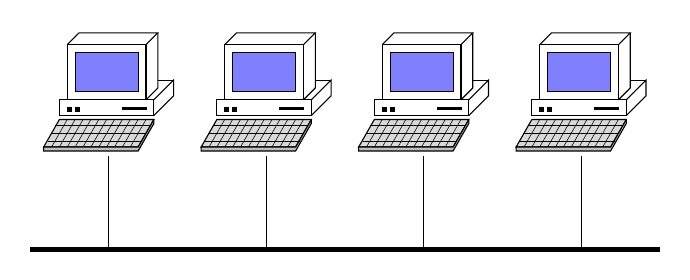
\begin{tikzpicture}
  \node[scale=0.5] (a) at (0,0) {\computertwo};
  \node[scale=0.5] (b) at (2,0) {\computertwo};
  \node[scale=0.5] (c) at (4,0) {\computertwo};
  \node[scale=0.5] (d) at (6,0) {\computertwo};
  \draw[ultra thick] (-1,-2) -- (7,-2);
  \foreach \from in {a,b,c,d} {
	 \draw (\from) -- ($(\from)+(0,-2)$);
  }
\end{tikzpicture}
\end{center}


\subsubsection{مزایا و معایب توپولوژی \lr{Bus}}

\begin{itemize}
	\item هزینه ی راه اندازی پایین 
	\item سرعت پایین، چون تنها یک مسیر وجود دارد
	\item تصادم اطلاعات باعث می شود داده ها از بین بروند
\end{itemize}


\newpage

\subsection{\lr{Ring}}

شبکه ای که از توپولوژی 
\lr{ring}
استفاده می کند ، کامپیوتر ها را در یک حلقه ی بسته به هم متصل می کند به این صورت که کابلی کامپیوتر اول را به کامپیوتر دوم متصل می کند ، کابل دیگری کامپیوتر دوم را به کامپیوتر سوم متصل می کند و این روال به همین ترتیب ادامه می باشد تا زمانی که کابلی کامپیوتر آخر را به اولین کامپیوتر متصل کند .

بعضی از تکنولوژی ها برای پیاده سازی توپولوژی 
\lr{ring}
نیاز به این دارند که کامپیوتر به دستگاه کوچکی متصل شود ، مزیت استفاده از یک دستگاه مجزا این است که حتی اگر کامپیوتری ارتباط خود را از شبکه قطع کند ، حلقه همچنان پابرجاست


\begin{center}
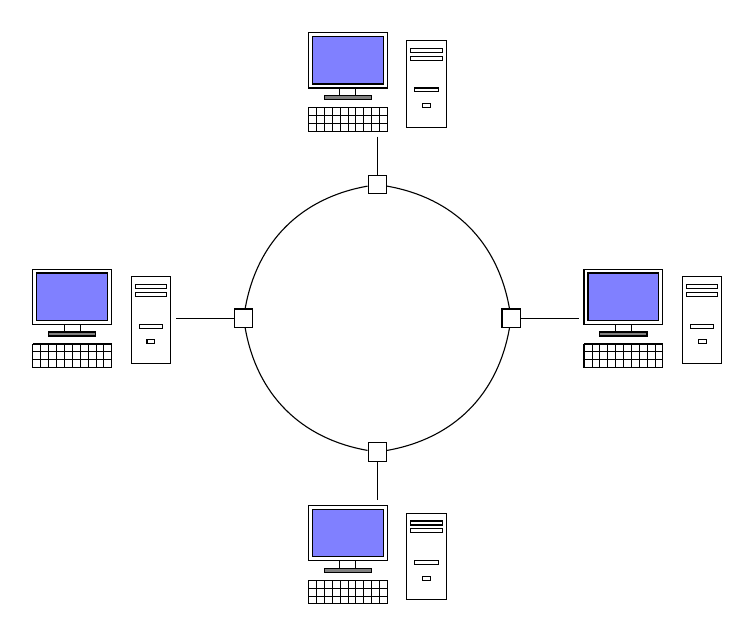
\begin{tikzpicture}
  \node[scale=0.5] (a) at (-0.5,0) {\computer};
  \node[scale=0.5] (b) at (3,3) {\computer};
  \node[scale=0.5] (c) at (6.5,0) {\computer};
  \node[scale=0.5] (d) at (3,-3) {\computer};
  \node[draw] (aa) at (1.3,0) {};
  \node[draw] (bb) at (3,1.7) {};
  \node[draw] (cc) at (4.7,0) {};
  \node[draw] (dd) at (3,-1.7) {};
  \draw (a) -- (aa);
  \draw (b) -- (bb);
  \draw (c) -- (cc);
  \draw (d) -- (dd);
  \draw (aa) edge[bend left=35] (bb);
  \draw (bb) edge[bend left=35] (cc);
  \draw (cc) edge[bend left=35] (dd);
  \draw (dd) edge[bend left=35] (aa);
\end{tikzpicture}
\end{center}


\subsubsection{مزایا و معایب توپولوژی \lr{Star}}

\begin{itemize}
	\item پهنای باند افزایش می یابد
	\item اضافه و حذف کردن کامپیوترها آسان است
\end{itemize}


\newpage

\subsection{\lr{Mesh}}

توپولوژی 
\lr{mesh}
بین هر دو کامپیوتر که در شبکه وجود دارد ارتباط مستقیم برقرار می کند ، هزینه ی بالا عیب بزرگ این توپولوژی می باشد .

شبکه ی 
\lr{mesh}
ای که 
\lr{n}
کامپیوتر را به هم متصل می کند ، به تعداد

\begin{tcolorbox}
$$
\cfrac{n!}{(n-2)!2!} = \cfrac{n^{2} - n}{2}
$$
\end{tcolorbox}

\lr{connection}
نیاز دارد


نکته ی مهمی که مشاهده می شود این است که تعداد
\lr{connection}
هایی که برای توپولوژی 
\lr{mesh}
استفاده می شود از تعداد کامپیوتر های شبکه رشد بیشتری دارد و از آنجایی که هزینه ی برقراری هر ارتباط بالاست بنابراین
\lr{LAN}
های کمتری از توپولوژی 
\lr{mesh}
استفاده می کنند



\begin{center}
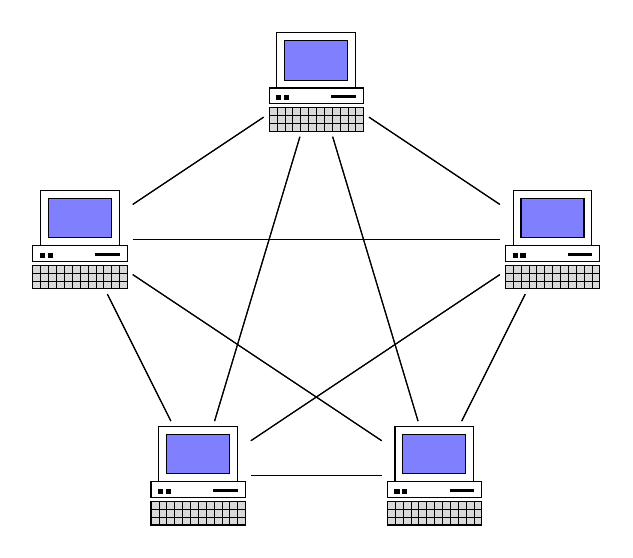
\begin{tikzpicture}
  \node[scale=0.5] (a) at (0,0) {\computerthree};
  \node[scale=0.5] (b) at (1.5,-3) {\computerthree};
  \node[scale=0.5] (c) at (4.5,-3) {\computerthree};
  \node[scale=0.5] (d) at (6,0) {\computerthree};
  \node[scale=0.5] (e) at (3,2) {\computerthree};
  \foreach \from in {a,b,c,d,e} {
  	\foreach \to in {a,b,c,d,e} {
	    \draw (\from) -- (\to);
	}
  }
\end{tikzpicture}
\end{center}


\newpage

\subsection{\lr{Star}}

یک شبکه با توپولوژی
\lr{star}
همه ی کامپیوتر ها را به یک نقطه ی مرکزی متصل می کند ،
از آنجایی که شکل توپولوژی 
\lr{star}
شبیه بک چرخ می باشد ،
مرکز چنین شبکه هایی
\lr{hub}
نامیده می شود .

\lr{hub}
یک دستگاه الکترونیکی است ، که اطلاعات را از کامپیوتر فرستنده دریافت می کند و به مقصد مورد نظر تحویل می دهد .


\begin{center}
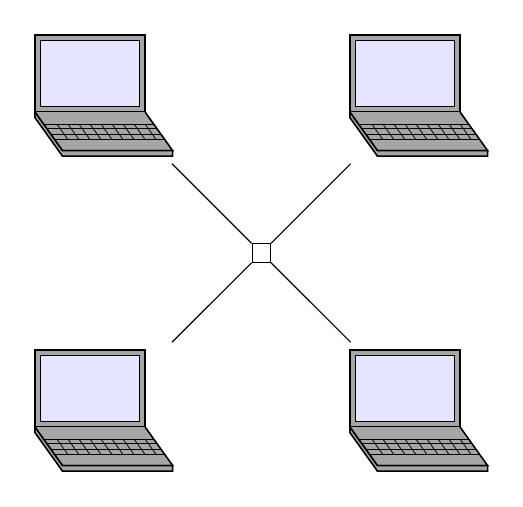
\begin{tikzpicture}
  \node[scale=0.7] (a) at (-2,2) {\laptop};
  \node[scale=0.7] (b) at (2,2) {\laptop};
  \node[scale=0.7] (c) at (-2,-2) {\laptop};
  \node[scale=0.7] (d) at (2,-2) {\laptop};
  \node[draw] (center) at (0,0) {};
  \foreach \from in {a,b,c,d} {
	\draw (\from) -- (center);
  }
\end{tikzpicture}
\end{center}



\section{سخت افزار های ایجاد شبکه}


\subsection{\lr{Hub}}

\lr{hub}
یک سخت افزار شبکه برای ارتباط بین چندین دستگاه به یکدیگر است که باعث می شود همه ی آنها به عنوان یک مجموعه در نظر گرفته شوند .

\lr{hub}
دارای چندین 
\lr{port}
ورودی-خروجی است که در آن سیگنالی که به عنوان ورودی در یک 
\lr{port}
خاصی دریافت می شود به همه ی 
\lr{port}
های دیگر به غیر از خودش ارسال می شود .




\begin{center}
	\includegraphics[scale=0.6]{./network-hubs-500x500.jpg}
	%\caption{}
\end{center}

\subsection{\lr{Switch}}

\lr{switch}
در شبکه یک دستگاه الکترونیکی پرسرعت است که اطلاعات را از ورودی دریافت می کند و به سمت مقصد ارسال می کند .

\lr{hub}
و
\lr{switch}
از لحظ شکل ظاهری بسیار شبیه به هم می باشند .

\begin{center}
	\includegraphics[scale=0.6]{./d-link-32-code-networking-switch-500x500.png}
	%\caption{}
\end{center}



\subsubsection{تفاوت
\lr{switch}
و
\lr{hub}
}

در 
\lr{hub}
اطلاعات دریافت شده بدون توجه به آدرس مقصد به همه ی 
\lr{port}
های دیگر به غیر 
\lr{port}
دریافتی ارسال می شود ،
ولی در 
\lr{switch}
اطلاعات فقط به 
\lr{port}
ای ارسال می شود که در آدرس مقصد تعیین شده است .


\subsection{\lr{Router}}

\lr{router}
سخت افزار شبکه است که تعدادی ورودی و خروجی دارد و بسته های اطلاعاتی را از ورودی ها تحویل گرفته و بر اساس آدرس مقصد یکی از کانال های خروجی را برای ارسال اطلاعات انتخاب نماید به طوری که بسته را به مقصد نزدیک نماید در واقع
\lr{router}
عملکرد هدایت و مسیریابی اطلاعات را در اینترنت بر عهده دارد که با استفاده از جدول مسیریابی که در خود دارد ، تصمیم میگیرد که اطلاعات را به کدام شبکه ی بعدی بفرستد .


\begin{center}
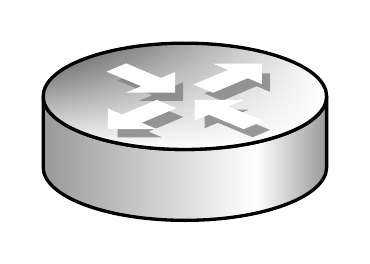
\begin{tikzpicture}
  \node[scale = 1.5] (a) {\router{}};
\end{tikzpicture}
\end{center}



\subsubsection{میزبان \lr{(Host)}}

عضوی از شبکه است که هیچ نقشی در هدایت بسته های اطلاعاتی در شبکه ندارد و فقط تولید کننده یا دریافت کننده بسته های اطلاعاتی است ، مثل : کامپیوتر شخصی یا تلفن همراه شما .


\subsubsection{\lr{Network Interface Controller (NIC)}}

کنترلگر واسط شبکه یا
\lr{Network Interface Controller}
یک سخت افزار کامپیوتری است که کامپیوتر را به شبکه متصل می کند .

\begin{center}
	\includegraphics[scale=0.3]{./640px-Network_card.jpg}
	%\caption{}
\end{center}

\section{\lr{MAC Address}}

\lr{MAC Address}
یک شناسه ی منحصر به قرد است که به کنترلگر واسط شبکه نسبت داده می شود و به عنوان آدرس سخت افزاری میزبان در شبکه مورد استفاده قرار می گیرد . نمونه ای از 
\lr{MAC Address}
به صورت زیر است .
\begin{latin}
\begin{tcolorbox}
\begin{center}
00:0a:95:9d:68:16
\end{center}
\end{tcolorbox}
\end{latin}

\section{اینترنت چیست؟}

اینترنت یک سیستم جهانی است که  شبکه های کامپیوتری را به هم متصل می کند .

در واقع اینترنت شبکه ای از شبکه هاست .

 
\section{\lr{IP Address}}

آدرس پروتکل اینترنتی یا
\lr{IP}
یک نماد عددی است که به هر دستگاه موجود در شبکه تخصیص داده می شود .

آدرس
\lr{IP}
به دو قسمت اصلی تقسیم می شود :
\begin{itemize}
	\item قسمت شبکه
	\item قسمت میزبان
\end{itemize}


\begin{center}
\begin{tikzpicture}
\draw[<->,>=latex] (0,0) -- node[above] { بیت 32 } (8,0);
\draw (0,-0.5) rectangle (4,-1.5);
\draw (4,-0.5) rectangle (8,-1.5);
\node at (2,-1) {شبکه کننده مشخص};
\node at (6,-1) {میزبان کننده مشخص};
\end{tikzpicture}
\end{center}

مزیت استفاده از مدل دو بخشی آدرس شبکه و آدرس میزبان برای آدرس های
\lr{ IP }
	، کمینه کردن تعداد ورودی ها در جدول مسیریابی است .
	به جای اینکه برای هر میزبان در یک شبکه یک رکورد در جدول مسیریابی داشته باشیم، میتوان با استفاده از یک رکورد همه ی میزبان ها را در یک شبکه خلاصه کرد که فقط شامل قسمت آدرس شبکه است که پیشوند مشترک برای همه ی میزبان های شبکه می باشد .


\section{انواع کلاسهای \lr{IP} }


\begin{itemize}
	\item \lr{Class A} با عدد $0$ شروع می شود 
\end{itemize}

\begin{align*}
 0.  0.  0.  0 = &\underbrace{00000000}_{Network}.\underbrace{00000000.00000000.00000000}_{Host} \\
127.255.255.255 = &\underbrace{01111111}_{Network}.\underbrace{11111111.11111111.11111111}_{Host} \\
                  &0nnnnnnn.HHHHHHHH.HHHHHHHH.HHHHHHHH
\end{align*}



\begin{itemize}
	\item \lr{Class B} با عدد $10$ شروع می شود 
\end{itemize}

\begin{align*}
128.  0.  0.  0 = &\underbrace{10000000.00000000}_{Network}.\underbrace{00000000.00000000}_{Host} \\
191.255.255.255 = &\underbrace{10111111.11111111}_{Network}.\underbrace{11111111.11111111}_{Host} \\
                  &10nnnnnn.nnnnnnnn.HHHHHHHH.HHHHHHHH
\end{align*}



\begin{itemize}
	\item \lr{Class C} با عدد $110$ شروع می شود 
\end{itemize}

\begin{align*}
192.  0.  0.  0 = &\underbrace{11000000.00000000.00000000}_{Network}.\underbrace{00000000}_{Host} \\
223.255.255.255 = &\underbrace{11011111.11111111.11111111}_{Network}.\underbrace{11111111}_{Host} \\
                  &110nnnnn.nnnnnnnn.nnnnnnnn.HHHHHHHH
\end{align*}




\begin{itemize}
	\item \lr{Class D} با عدد $1110$ شروع می شود 
\end{itemize}

\begin{align*}
224.  0.  0.  0 = &11100000.00000000.00000000.00000000 \\
239.255.255.255 = &11101111.11111111.11111111.11111111 \\
                  &1110XXXX.XXXXXXXX.XXXXXXXX.XXXXXXXX
\end{align*}






\begin{itemize}
	\item \lr{Class E} با عدد $11110$ شروع می شود 
\end{itemize}

\begin{align*}
240.  0.  0.  0 = &11110000.00000000.00000000.00000000 \\
255.255.255.255 = &11111111.11111111.11111111.11111111 \\
                  &1111XXXX.XXXXXXXX.XXXXXXXX.XXXXXXXX
\end{align*}






\section{خلاصه ی کلاس های IP به صورت جدول}

\begin{latin}
\begin{center}
  \rowcolors{1}{codepurple!70}{backcolour}
  \bgroup
  \def\arraystretch{1.5}%
  \begin{tabular}{ c  c  c  c  c    }
    Class & Starting Bits & Size of network ( bit) & Size of Host (bit) & \\
    \hline
    Class A & 0 & 8 & 24  & \\ \hline
   & \multicolumn{2}{c}{Number of networks} & \multicolumn{2}{c}{Hosts per Network}   \\ \hline
   & \multicolumn{2}{c}{128 $(2^{7})$} & \multicolumn{2}{c}{16,777,216 $(2^{24})$} \\ \hline
   & \multicolumn{2}{c}{Total addresses in class}  & Start address & End address   \\ \hline
   & \multicolumn{2}{c}{2,147,483,648 $(2^{31})$} & 0.0.0.0 & 	127.255.255.255  \\ \hline
  \end{tabular}
  \egroup
\end{center}
\end{latin}




\begin{latin}
\begin{center}
  \rowcolors{1}{codepurple!70}{backcolour}
  \bgroup
  \def\arraystretch{1.5}%
  \begin{tabular}{ c  c  c  c  c    }
    Class & Starting Bits & Size of network ( bit) & Size of Host (bit) & \\
    \hline
    Class B & 10 & 16 & 16 & \\ \hline
           & \multicolumn{2}{c}{Number of networks} & \multicolumn{2}{c}{Hosts per Network}   \\ \hline
          & \multicolumn{2}{c}{16,384 $(2^{14})$} & \multicolumn{2}{c}{65,536 $(2^{16})$}   \\ \hline
   & \multicolumn{2}{c}{Total addresses in class}  & Start address & End address  \\ \hline
   & \multicolumn{2}{c}{1,073,741,824 $(2^{30})$} & 128.0.0.0 & 	191.255.255.255  \\ \hline
  \end{tabular}
  \egroup
\end{center}
\end{latin}



\begin{latin}
\begin{center}
  \rowcolors{1}{codepurple!70}{backcolour}
  \bgroup
  \def\arraystretch{1.5}%
  \begin{tabular}{ c  c  c  c  c   }
    Class & Starting Bits & Size of network ( bit) & Size of Host (bit) & \\
    \hline
    Class C & 110 & 24 & 8 & \\ \hline
    & \multicolumn{2}{c}{Number of networks} & \multicolumn{2}{c}{Hosts per Network}   \\ \hline
    & \multicolumn{2}{c}{2,097,152 $(2^{21})$} & \multicolumn{2}{c}{256 $(2^{8})$}   \\ \hline
   & \multicolumn{2}{c}{Total addresses in class}  & Start address & End address  \\ \hline
   & \multicolumn{2}{c}{536,870,912 $(2^{29})$} & 192.0.0.0 & 	223.255.255.255   \\ \hline
  \end{tabular}
  \egroup
\end{center}
\end{latin}



\subsubsection{
 یک شبکه کلاس C با آدرس 
\lr{194.34.56.0}
داده شده است، چند میزبان برای  این شبکه وجود دارد ؟ 
}


\begin{tcolorbox}
\begin{align*}
194.34.56.0 \to \underbrace{11000010.00100010.00111000}_{Network}.\underbrace{00000000}_{Host}
\end{align*}

{
\LARGE
$$
2^{8} - 2
$$
}
\end{tcolorbox}



\subsubsection{
 یک شبکه کلاس B با آدرس 
\lr{166.23.0.0}
داده شده است، چند میزبان برای  این شبکه وجود دارد ؟ 
}

\begin{tcolorbox}
\begin{align*}
166.23.0.0 \to \underbrace{10100110.00010111}_{Network}.\underbrace{00000000.00000000}_{Host}
\end{align*}

{
\LARGE
$$
2^{16} - 2
$$
}
\end{tcolorbox}


\newpage

\subsubsection{مثال}


 مشخص کنید که آدرس 
\lr{192.168.1.18/24}
جزء کدام دسته کلاس آدرس می باشد و آدرس خود شبکه ، اولین میزبان ، آخرین میزبان و آدرس Broadcast را در این شبکه مشخص کنید ؟


\begin{itemize}
	\item آدرس خود شبکه آدرسی است که تمام بیت ها در قسمت میزبان برابر با صفر باشد
	\item آدرس 
\lr{Broadcast}
آدرسی است که تمام بیت ها در قسمت میزبان برابر با یک باشد
\end{itemize}



\begin{tcolorbox}
$$
192.168.1.18 \to 11000000.10101000.00000001.00010010 \Rightarrow class \:\: C
$$

$$
\underbrace{192.168.1}_{Network}.\underbrace{18}_{Host}
$$


\begin{align*}
Subnet &= 192.168.1.00000000 \\
1st \:\: Host &= 192.168.1.00000001 \\
Last \:\: Host &= 192.168.1.11111110 \\
Broadcast &= 192.168.1.11111111 \\
\end{align*}

\end{tcolorbox}




\newpage

\subsubsection{مثال}


 مشخص کنید که آدرس 
\lr{172.16.35.123/20}
جزء کدام دسته کلاس آدرس می باشد و آدرس خود شبکه ، اولین میزبان ، آخرین میزبان و آدرس
\lr{ Broadcast}
 را در این شبکه مشخص کنید ؟


\begin{itemize}
	\item آدرس خود شبکه آدرسی است که تمام بیت ها در قسمت میزبان برابر با صفر باشد
	\item آدرس 
\lr{Broadcast}
آدرسی است که تمام بیت ها در قسمت میزبان برابر با یک باشد
\end{itemize}




\begin{tcolorbox}
$$
172.16.35.123 \to 10101100.00010000.00100011.01111011 \Rightarrow class \:\: B
$$


$$
\underbrace{172.16}_{Network}.\underbrace{35.123}_{Host}
$$


\begin{latin}
\begin{center}
  \begin{tabular}{ r  r | l  }
    Subnet $\to$ & 172.16.0010 & 0000.00000000 \\
    1st Host $\to$ & 172.16.0010 & 0000.00000001 \\
    Last Host $\to$ & 172.16.0010 & 1111.11111110 \\
    Broadcast $\to$ & 172.16.0010 & 1111.11111111 \\
  \end{tabular}
\end{center}
\end{latin}


\begin{latin}
\begin{center}
  \begin{tabular}{ r  l   }
    Subnet $\to$ & 172.16.32.0  \\
    1st Host $\to$ & 172.16.32.1  \\
    Last Host $\to$ & 172.16.47.254 \\
    Broadcast $\to$ & 172.16.47.255 \\
  \end{tabular}
\end{center}
\end{latin}

\end{tcolorbox}





\newpage

\subsubsection{مثال}


 مشخص کنید که آدرس 
\lr{172.16.129.1/17}
جزء کدام دسته کلاس آدرس می باشد و آدرس خود شبکه ، اولین میزبان ، آخرین میزبان و آدرس
\lr{ Broadcast}
 را در این شبکه مشخص کنید ؟


\begin{tcolorbox}
$$
172.16.129.1 \to 10101100.00010000.10000001.00000001 \Rightarrow class \:\: B
$$


$$
\underbrace{172.16}_{Network}.\underbrace{129.1}_{Host}
$$



\begin{latin}
\begin{center}
  \begin{tabular}{ r  r | l  }
    Subnet $\to$ & 172.16.1 & 0000000.00000000 \\
    1st Host $\to$ & 172.16.1 & 0000000.00000001 \\
    Last Host $\to$ & 172.16.1 & 1111111.11111110 \\
    Broadcast $\to$ & 172.16.1 & 1111111.11111111 \\
  \end{tabular}
\end{center}
\end{latin}



\begin{latin}
\begin{center}
  \begin{tabular}{ r  l   }
    Subnet $\to$ & 172.16.128.0  \\
    1st Host $\to$ & 172.16.128.1  \\
    Last Host $\to$ & 172.16.255.254 \\
    Broadcast $\to$ & 172.16.255.255 \\
  \end{tabular}
\end{center}
\end{latin}

\end{tcolorbox}




\newpage


\section{ساختار \lr{IPv4}}

\begin{center}
	\includegraphics[scale=0.6]{./ip_1.png}
	%\caption{}
\end{center}


یک بسته آی پی از دو بخش سرآیند
\lr{(header)}
 و داده تشکیل می‌شود
 
\subsection{سرآیند \lr{(header)}}

سرآیند بسته 
\lr{IPv4}
 از 13 فیلد تشکیل می‌شود که 12 تای آن‌ها اجباری هستند. فیلد سیزدهم اختیاری است. این فیلدها به گونه‌ای در سرآیند بسته‌بندی می‌شوند که پرارزش‌ترین بایت در ابتدا بیاید. 

\subsubsection{شماره نسخه}
نسخه: اولین فیلد در سرآیند یک بسته 
\lr{IP}
 ، فیلد 4 بیتی نسخه‌است. مقدار این فیلد برای بسته 
 \lr{IP}
نسخه چهار، 4 می‌باشد.


\subsubsection{طول سرآیند}

این فیلد طول سرآیند بسته را بر حسب تعداد کلمه های 32 بیتی مشخص می‌کند. از آنجا که در یک بسته 
\lr{IP}
نسخه 4 طول فیلد اختیاری ثابت نیست، اندازه سرآیند در این فیلد ذخیره می‌شود (که برابر با محل شروع فیلد داده نیز هست). کمترین مقدار مجاز برای این فیلد 5 است 
\lr{(RFC 791) }
که برابر با
 $32\times5=160$ 
 بیت می‌باشد. و از آنجا که این فیلد 4بیتی است بیشترین مقدار آن 15 کلمه یا
$32\times15= 480$
  بیت است.



\subsubsection{فیلد نوع سرویس}

فیلد نوع سرویس ، نوع سرویس دریافتی را از نظر پارامترهایی نظیر :

\begin{itemize}
	\item میزان تقدم
	\item تاخیر
	\item گذردهی
	\item اطمینان
\end{itemize}
مشخص می کند .


\subsubsection{فیلد طول کلی}

فیلد طول کلی نشان دهنده ی طول بسته ی 
\lr{IP}
شامل سرآیند
\lr{IP}
و داده بر حسب بایت می باشد .
این فیلد 16 بیت طول دارد .


\subsubsection{فیلد شناسایی}

فیلد شناسایی برای هر بسته به طور یکتا مقدار دهی می شود و نشان دهنده ی شماره ی بسته می باشد .

\subsubsection{فیلد پرچم}

فیلد پرچم 3 بیت طول دارد . اولین بیت این فیلد همواره صفر است . بیت های دوم و سوم به ترتیب بیت های
\lr{DF}
و
\lr{MF}
می باشند .

اگر مقدار پرچم
\lr{DF}
برابر با 1 باشد ، به این معنی است که نباید بسته تکه سازی شود .

چنانچه پرچم 
\lr{MF}
برابر با 1 باشد ، گیرنده متوجه خواهد شد که تمام تکه های بسته اصلی هنوز نیامده اند و تکه های دیگری در راه می باشند .






\subsubsection{زمان زندگی \lr{(TTL)}}

فیلد زمان زندگی که بر حسب ثانیه اندازه گیری می شود نشان دهنده ی حداکثر زمانی است که یک بسته 
\lr{IP}
می تواند در شبکه زنده بماند .
 این فیلد 8 بیتی از باقی ماندن بسته‌های سرگردان 
 \lr{IP}
  در شبکه جلوگیری می‌کند. مقدار این بسته توسط پیش‌فرض سیستم تعیین می‌شود و پس از عبور از هر مسیریاب یک شماره از این فیلد کم می‌شود. اگر این مقدار صفر شود مسیریاب بسته را حذف می‌کند و یک پیام
  \lr{ ICMP}
   به فرستنده بسته می‌فرستد و فرستنده متوجه می‌شود که عمر بسته پایان یافته‌است.


\subsubsection{فیلد پروتکل}

فیلد پروتکل برای مشخص کردن پروتکل لایه بالایی که باید داده های موجود در بسته
\lr{IP}
را دریاقت کند ، استفاده می شود .


\subsubsection{مجموع مقابله‌ای سرآیند \lr{ (Header Checksum)}}

این فیلد  16 بیتی برای کشف خطا به کار می‌رود. در هر جهش (hop) باید مجموع مقابله‌ای سرآیند محاسبه و با مقدار این فیلد مقایسه شود. اگر این دو مقدار برابر نباشند به معنی بروز خطای انتقال است و بسته حذف می‌شود .
نحوه ی محاسبه به این صورت است که مکمل 1 تمام مقادیر 16 بیتی موجود در سرآیند 
\lr{IP}
با هم جمع می شوند ( به جز خود فیلد مجموع مقابله ای سرآیند ) ، سپس مکمل 1 مجموع محاسبه می شود ،اگر این دو مقدار با هم برابر باشند به معنی عدم وجود خطا در بسته می باشد . هر دو پروتکل UDP و TCP ، فیلد مجموع مقابله‌ای دارند.


\subsubsection{فیلد گزینه و فیلد \lr{padding}}

از فیلد گزینه برای فراهم سازی برخی امکانات اضافی در پروتکل 
\lr{IP}
استفاده می شود 

چنانچه طول فیلد گزینه مضربی از 4 نبوده ، به مقدار کافی در ناحیه ی
 padding 
بیت صفر اضافه می شود تا فیلد گزینه مضربی از 32 بیت باشد .

\section{انواع پروتکل ها در شبکه}

\subsection{\lr{DNS}}

\lr{DNS}
مخفف
\lr{Domain Name System}
یک سیستم سلسه‌مراتبی نام‌گذاری برای کامپیوترها، سرویس‌ها، یا منابع دیگر است که به شبکه اینترنت متصل هستند .

وقتی می خواهید وارد سایتی شوید باید آدرس 
\lr{IP}
آن را بدانید اما چون به خاطر سپردن آدرس های 
\lr{IP} 
دشوار است ، هر آدرس 
\lr{IP}
به نام مخصوصی نگاشته می شود .

کل نشانی‌های اینترنت درون بانک‌های اطلاعاتی توزیع شده‌ای هستند که هیچ تمرکزی روی نقطه‌ای خاص از شبکه ندارند. 

روش ترجمهٔ نام بدین صورت است که وقتی یک برنامهٔ کاربردی مجبور است برای برقراری یک ارتباط، معادل نشانی آی‌پی از یک ماشین با نامی مثل
\lr{ cs.ucsb.edu }
 را بدست بیاورد، قبل از هر کاری یک تابع کتابخانه‌ای را صدا می‌زند، به این تابع کتابخانه‌ای تابع تحلیلگر، نام 
\lr{ (Name Resolver) }
 گفته می‌شود. 
 
 تابع تحلیلگر، نام یک نشانی نمادین را که بایستی ترجمه شود، به عنوان پارامتر ورودی پذیرفته و سپس یک بستهٔ درخواست
\lr{ (Query Packet)  }
  به روش
\lr{ UDP  }
   تولید کرده و به نشانی یک کارساز
\lr{ DNS }
   (که به صورت پیش‌فرض مشخص می‌باشد) ارسال می‌کند. همهٔ ماشین‌های میزبان، حداقل باید یک نشانی آی‌پی از یک سرویس دهندهٔ ساناد را در اختیار داشته باشند. این «سرویس دهندهٔ محلی» پس از جستجو، نشانی آی‌پی معادل با یک نام نمادین را برمی‌گرداند.
   
«تابع تحلیلگر نام» نیز آن نشانی آی‌پی را به برنامهٔ کاربردی تحویل می‌دهد با پیدا شدن نشانی آی‌پی، برنامهٔ کاربردی می‌تواند عملیات مورد نظرش را ادامه دهد. 

\subsubsection{روش‌های جستجو}

همانگونه که اشاره شد، اسامی نمادین در شبکه اینترنت که خود در قالب حوزه‌ها و زیر حوزه‌ها سازماندهی شده‌اند، در یک فایل متمرکز ذخیره نمی‌شوند بلکه روی کل شبکه اینترنت توزیع شده‌اند، به همین دلیل برای ترجمه یک نام به نشانی آی‌پی ممکن است چندین مرحله «پرس و جو» صورت بگیرد تا یک نشانی پیدا شود.

طبیعی است که یک پرس و جو برای تبدیل یک نام حوزه همیشه موفقیت‌آمیز نباشد و ممکن است به پرس و جوهای بیشتری نیاز شود یا حتی ممکن است یک نشانی نمادین اشتباه باشد و هیچ معادل نشانی آی‌پی نداشته باشد.

سه روش برای پرس و جوی نام در سرویس دهنده‌های نام وجود دارد :

\begin{itemize}
	\item پرس و جوی تکراری \lr{Iterative Query}
	\item پرس و جوی بازگشتی \lr{Recursive Query}
	\item پرس و جوی معکوس \lr{Reverse Query}
\end{itemize}


\subsubsection{پرس و جوی تکراری}

در پرس و جوی تکراری قسمت اعظم تلاش برای تبدیل یک نام بر عهده سرویس دهنده محلی است؛ این DNS حداقل به نشانی ماشین Root، به عنوان نقطه شروع نیاز دارد. وقتی یک تقاضای ترجمه نشانی به سرویس دهنده محلی ارسال می‌شود در صورتی که قادر به ترجمه نام به معادل نشانی آی‌پی آن باشد، معادل نشانی آی‌پی نام مورد نظر را به تقاضاکننده برمی‌گرداند. (این حالت وقتی است که سرویس دهنده محلی قبلاً آن نام را ترجمه و در یک فایل ذخیره کرده باشد) در غیر این صورت سرویس دهنده محلی خودش یک تقاضا برای DNS سطح بالا ارسال می‌کند. این سرویس دهنده، نشانی ماشینی را که می‌تواند برای ترجمه نام مورد نظر مفید باشد، به سرویس دهنده محلی معرفی می‌کند؛ سرویس دهنده محلی مجدداً یک تقاضا به ماشین معرفی شده در مرحله قبل ارسال می‌کند. 


\subsubsection{پرس و جوی بازگشتی}


در این روش هر گاه برنامه‌ای بخواهد نشانی آی‌پی معادل یک نام مثل cs.yale.edu را بدست آورد، بگونه‌ای که قبلاً اشاره شد، «تابع سیستمی تحلیل نام» را فراخوانی می‌کند. این تابع یک ماشین را به عنوان سرویس دهنده محلی از قبل می‌شناسد و بنابراین تقاضای تبدیل نام را به روش UDP برای آن ارسال کرده و منتظر جواب می‌ماند (پاسخ نهایی DNS طبیعتاً باید یک نشانی ۳۲ بیتی معادل نشانی آی‌پی یک ماشین باشد)

دو حالت ممکن است اتفاق بیفتد:

ممکن است در بانک اطلاعاتی مربوط به سرویس دهنده محلی، نشانی آی‌پی معادل با آن نام از قبل وجود داشته و بالطبع به سرعت مقدار معادل نشانی آی‌پی آن بر می‌گردد. ممکن است در بانک اطلاعاتی سرویس دهنده محلی، معادل نشانی آی‌پی آن نام وجود نداشته باشد. مثلاً سرویس دهنده محلی در بانک اطلاعاتی خودش معادل نشانی آی‌پی نام cs.mit.edu را نداشته و طبیعتاً نمی‌تواند آن را ترجمه کند.

در چنین حالتی سرویس دهنده محلی موظف است بدون آنکه به تقاضا دهنده خبر بدهد، خودش رأساً به سرویس دهنده سطح بالاتر تقاضای ترجمه نشانی بدهد. در این حالت هم DNS سطح بالاتر به همین نحو، ترجمه نشانی را پیگیری می‌کند. یعنی اگر معادل نشانی آی‌پی آن نام را داشته باشد آن را برمی‌گرداند و در غیر اینصورت خودش از سرویس دهنده سطح پایینتر تقاضای ترجمه آن نام را می‌نماید و این مراحل تکرار می‌شود. در روش پرس و جوی بازگشتی ماشین سرویس دهنده محلی این مراحل متوالی را نمی‌بیند و هیچ کاری جز ارسال تقاضای ترجمه یک نشانی بر عهده ندارد و پس از ارسال تقاضا برای سرویس دهنده سطح بالا منتظر خواهد ماند.

بازهم تکرار می‌کنیم، روشی که DNS برای ترجمه نشانی بکار می‌برد می‌تواند بدون اتصال (UDP) باشد که این کار به سرعت عمل ترجمه نشانی می‌افزاید.

دقت کنید که در روش پرس و جوی تکراری نسبت به روش پرس و جوی بازگشتی، حجم عمده عملیات بر عهده سرویس دهنده DNS محلی است و مدیریت خطاها و پیگیری روند کار ساده‌تر خواهد بود و روش منطقی تری برای بکارگیری در شبکه اینترنت محسوب می‌شود. روش پرس و جوی بازگشتی برای شبکه‌های کوچک کاربرد دارد.


\subsubsection{پرس و جوی معکوس}

فرض کنید حالتی بوجود بیاید که یک سرویس دهنده DNS، نشانی آی‌پی یک ماشین را بداند ولی نام نمادین معادل با آن را نداند.

در چنین حالتی مسئله کمی حادتر به نظر می‌رسد، چرا که برای ترجمه نامهای نمادین، چون این نامها دارای حوزه و زیرحوزه هستند، تحلیل نشانی‌ها ساده‌است؛ ولی ترجمه نشانی آی‌پی به معادل نام حوزه، از چنین روابطی تبعیت نمی‌کند؛ بعبارت بهتر هیچ ارتباط مستقیم و متناظری بین نشانی‌های آی‌پی و اسامی انتخاب شده در اینترنت وجود ندارد. برای یافتن نامهای متناظر با یک نشانی آی‌پی باید یک جستجوی کامل و در عین حال وقت گیر، انجام بشود.

روش کار بدین صورت است که سرویس دهنده محلی یک تقاضا برای DNS متناظر با شبکه‌ای که مشخصه آن در نشانی آی‌پی، مشخص شده، ارسال می‌کند. 


\subsection{\lr{ICMP}}

یکی از پروتکل‌های اصلی بستهٔ پروتکل‌های اینترنت می‌باشد. مورد اصلی استفاده از آن در سیستم عاملهای کامپیوترهای متصل به شبکه، برای ارسال پیام‌های خطا .


\begin{center}
	\includegraphics[scale=0.5]{./icmp_1.png}
	%\caption{}
\end{center}




\lr{ICMP}
متکی بر 
\lr{IP}
برای انجام کارهای خود است، و خودبخشی جدایی ناپذیر از 
\lr{IP}
 می‌باشد.
 
از جمله خطاهایی که میتوان برای ارسال آن از
\lr{ ICMP }
استفاده کرد ، می توان به موارد زیر اشاره کرد .
 
 \begin{itemize}
	\item صفر شدن TTL
	\item عدم تحویل بسته به علت گم شدن یک تکه از بسته
	\item در دسترس نبودن یک پروتکل ، سرویس یا میزبان خاص در مقصد
	\item عدم توانایی پیش بردن یک بسته به خاطر عدم اجازه تکه سازی
	\item وقوع ازدحام در یک مسیریاب شبکه
\end{itemize}
 
 پیام های
\lr{ ICMP }
برای اعلام وقوع خطا برای خود پیام های
\lr{ ICMP }
استفاده نمی شوند . زیرا پیام ها به شدت زیاد شده و به ترافیک شبکه اضافه می شود .
 
 
  هنگامی که یک مسیریاب شبکه بسته ای را برای ارسال دریافت نماید ولی تشخیص دهد که مسیریاب دیگری مسیر بهینه تری برای ارسال بسته به سمت مقصد دارد ، 
	اقدام به ارسال پیام 
\lr{ ICMP }
	 تغییر مسیر می نماید .

\subsubsection{
در حالت های زیر پیام ICMP تخطی زمانی فرستاده می شود .
}

\begin{itemize}
	\item هر گاه مقدار فیلد TTL در بسته های IP به صفر برسد 
	\item هرگاه یک تکه از بسته های IP
	 تکه شده طی زمان مشخصی به مقصد   نرسد ،
 مقصد یک پیام
	 ICMP تخطی زمانی 
	با مقدار کد 1 ارسال می کند
\end{itemize}


\subsubsection{
پیام ICMP مشکل پارامتر 
}

\begin{itemize}
	\item چنانچه مسیریاب متوجه مشکلی در پارامترهای سرآیند IP بسته های دریافتی شوند ،
	از پردازش بسته جلوگیری کرده و یک پیام ICMP 
	مشکل پارامتر ارسال می شود .
\end{itemize}



\subsubsection{
پیام ICMP فرونشاندن مبدا 
}

\begin{itemize}
	\item هنگامی که یک مسیریاب متوجه پر شدن ظرفیت حافظه ی خود می شود ، برای کاهش درخواست ها و کاهش ازدحام شبکه با حذف بسته های ورودی اضافی و فرستاده پیام ICMP فرو نشاندن مبدا به فرستندهایی که بیشترین درخواست ها را می فرستد از آن می خواهد که سرعت ارسال اطلاعات خود را کاهش دهند .
\end{itemize}




پیام های 
\lr{ ICMP }
برای ارسال 
از بسته های 
\lr{IP}
استفاده می کنند 
، و چون پروتکل 
\lr{IP}
تحویل پیام ها را ضمانت نمی کند بنابراین ممکن است پیام های 
\lr{ ICMP }
گم شده و یا به خاطر ازدحام در مسیریاب های میانی حذف شوند .



\subsection{\lr{ARP}}

\lr{Address Resolution Protocol}
یک پروتکل ارتباطی برای یافتن آدرس لایه پیوند، مانند 
\lr{MAC Address}
 ، و ارتباطش با آدرس لایهٔ شبکه
\lr{ (IPv4) }
است.


\subsubsection{ کاربرد و دلیل استفاده از پروتکل \lr{ARP} }

\begin{itemize}
	\item از آنجاییکه در کامپیوتر مقصد، ابتدا لایه ی دوم قاب را از شبکه برداشته و بعد به لایه ی سوم که پروتکل IP 
	است تحویل می دهد ، لذا دانستن تنها آدرس IP مقصد کفایت نکرده و باید آدرس سخت افزاری کامپیوتر مقصد نیز داشته باشیم ، به این علت از پروتکلی به نام ARP استفاده می کنیم . 
	از پروتکل ARP 
	برای استخراج آدرس لایه سخت افزاری که به آن
	MAC-Address
	گفته می شود از آدرس IP استفاده می شود .
\end{itemize}


\begin{center}
	\includegraphics[scale=0.5]{./arp_1.png}
	%\caption{}
\end{center}


\subsubsection{محدودیت پروتکل \lr{ARP} }

\begin{itemize}
	\item پروتکل ARP
	توسط پروتکل IP بسته بندی نمی شود ، بلکه مستقیماً توسط پروتکل لایه پیوند داده بسته بندی می گردد . این بدان معنی است که پیام های پروتکل ARP را نمی توان مسیریابی کرد، یعنی نمی تواند از مرز یک مسیریاب عبور کند .
\end{itemize}



\subsubsection{
به چه علت پیام درخواست ARP به صورت همه پخشی ارسال می شود ؟
}

\begin{itemize}
	\item در هنگام ارسال پیام درخواست ARP
	از آنجاییکه آدرس سخت افزاری مقصد هنوز معلوم نیست، بنابراین درخواست فوق در لایه ی دوم به صورت همه پخشی ارسال شده طوری که همه ی میزبان های شبکه بتوانند آن را دریافت کنند .
\end{itemize}



\subsubsection{
 آیا پیام پاسخ ARP به صورت همه پخشی ارسال می شود ؟ توضیح دهید ؟
}


\begin{itemize}
	\item پاسخ ARP 
	که توسط نود مقصد فرستاده می شود یک قاب همه پخشی نیست ، زیرا این نود آدرس سخت افزاری را در پیام درخواست ARP دریافت کرده است . بنابراین در هنگام پاسخ دهی ، قاب پاسخ را به صورت تک پخشی ارسال می دارد .
\end{itemize}


\subsubsection{
 چگونه آزمون آدرس IP تکراری ARP انجام می شود ؟
}

\begin{itemize}
	\item هر کامپیوتر در هنگام راه اندازی یک درخواست ARP
	را در شبکه منتشر می کند . در این پیام آدرس IP مقصد مساوی با آدرس IP فرستنده می باشد .
	در صورتی که فرستنده پاسخ پیام ARP 
	را دریافت کند ، بدین معنی است که نود دیگری با این آدرس موجود می باشد که به معنای وجود آدرس های IP تکراری در شبکه می باشد .
\end{itemize}






\subsection{\lr{TCP}}


\begin{center}
	\includegraphics[scale=0.6]{./tcp_1.png}
	%\caption{}
\end{center}


\lr{Transmission Control Protocol}
که قرارداد کنترل انتقال یا پروتکل کنترل انتقال نیز گفته می‌شود؛ مجموعه‌ای از پروتکل‌های قراردادی است که پایه و اساس اینترنت می‌باشد. 

برای برقراری یک ارتباط گفتاری به وسیلهٔ اینترنت، در لایه انتقال از دو پروتکل TCP و UDP استفاده می‌شود. پروتکل TCP انتقال داده را با دقت و امنیت بالا انجام می‌دهد در حالیکه ویژگی پروتکل UDP انتقال سریع اطلاعات، بدون در نظر گرفتن اطمینان برای انتقال داده است 


مهمترین وظیفه پروتکل TCP اطمینان از صحت ارسال اطلاعات است. پروتکل فوق اصطلاحاً «ارتباط اتصال‌گرا» نامیده می‌شود. علت این امر ایجاد یک ارتباط مجازی بین کامپیوترهای فرستنده و گیرنده، قبل از ارسال اطلاعات است. پروتکل‌هایی از این نوع، امکانات بیشتری را به منظور کنترل خطاهای احتمالی در ارسال اطلاعات فراهم نموده ولی به دلیل افزایش بار عملیاتی سیستم، کارایی آنان کاهش خواهد یافت. از پروتکل TCP به عنوان یک پروتکل قابل اطمینان نیز یاد می‌شود. به این علت که برای آگاهی از صحت اطلاعات ارسال شده، اطلاعات دیگری نیز به گیرنده فرستاده می‌شود. در صورتی که بسته‌های اطلاعاتی به درستی دراختیار فرستنده قرار نگیرند ، فرستنده مجدداً اقدام به ارسال اطلاعات می‌نماید. 


\subsubsection {
 ویژگی های اصلی TCP را نوشته و به اختصار توضیح دهید ؟
}

\begin{itemize}
	\item حمل داده پایه ای
	\begin{itemize}
		\item[*] TCP توانایی حمل جریان پیوسته ای از بایت ها در هر دو جهت اتصال را دارد .
	\end{itemize}
	\item اطمینان
	\begin{itemize}
		\item[*] یکی از ویژگی های TCP تحویل مطمئن داده ها
		به صورت انتها به انتها است . برای مهیا سازی اطمینان TCP برای جبران داده های خراب ، گم شده از مدل ارسال مجدد تصدیق مثبت استفاده می نماید . در TCP سگمنت های جدید تنها زمانی فرستاده می شوند که سگمنت های قبلی ارسال شده تصدیق شده باشند . 
		\item[*] در TCP 
		فرستنده با ارسال هر سگمنت ، منتظر دریافت پیام تصدیق مثبت ( ACK ) از طرف گیرنده می باشد . اگر ACK
		در یک بازه زمانی معین دریافت نشود ، سگمنت قبلی دوباره ارسال می شود .
		\item[*] در TCP
		از مکانیزم شماره گذاری رشته برای مرتب کردن سگمنت هایی که خارج از نوبت دریافت شده اند و یا حذف سگمنت های تکراری استفاده می شود .
		\item[*] در TCP
		در صورت وقوع خرابی در سگمنت های دریافتی ، با استفاده از فیلد مجموع مقابله ای در سرآیند بسته های TCP 
		، مشکل رفع می شود .
	\end{itemize}
	\item کنترل جریان
	\begin{itemize}
		\item[*] توسط مکانیزم کنترل جریان در TCP
		، مقدار داده ارسال شده توسط فرستنده همواره کنترل می شود .
		\item[*] پروتکل TCP از مکانیزم پنجره ی لغزان
		برای پیاده سازی کنترل جریان استفاده می کند .
	\end{itemize}
	\item تسهیم سازی
	\begin{itemize}
		\item[*] استفاده مشترک چندین فرآیند لایه کاربرد از امکانات TCP/IP ، 
		تسهیم سازی نام دارد .
	\end{itemize}
	\item اتصال انتها به انتها
	\item تقدم و امنیت
\end{itemize}



\subsubsection{
 کاربرد فیلد های شماره رشته ارسال و شماره تصدیق را در بسته های TCP توضیح دهید ؟
}


\begin{itemize}
	\item شماره رشته نشان دهنده ی اولین بایت داده در یک سگمنت TCP ارسالی می باشد .
	\item شماره تصدیق نشان دهنده ی  شماره بایتی است که فرستنده ، انتظار دریافت آن از طرف مقابل را دارد .
	\item به عنوان مثال ، اگر فیلد شماره رشته 100 باشد و فیلد شماره تصدیق 200 باشد ، بدان معنی است که بسته ارسالی از بایت 100 به بعد را شامل می شود و فرستنده تا بایت 199 را به طرف مقابل می فرستد و منتظر بایت 200 به بعد از طرف مقابل می باشد .
\end{itemize}




\subsubsection{
 کاربرد هر یک از پرچم های TCP را توضیح دهید ؟
}


\begin{itemize}
	\item [\lr{ACK}] هنگامی که
	\lr{ACK}
، 	1 باشد نشان می دهد که فیلد شماره تصدیق معتبر است .
	\item [\lr{SYN}] برای نشان دادن باز شدن یک اتصال استفاده می شود
	\item [\lr{FIN}] برای قطع یک اتصال استفاده می شود
	\item [\lr{RST}] چنانچه در یک اتصال
	\lr{TCP}
	خطای غیر قابل ترمیمی رخ دهد ، از بیت
	\lr{ RST }
	برای درخواست ری ست اتصال استفاده می شود .
	\item [\lr{PSH}] وقتی این پرچم برابر با 1 شود
	گیرنده پیام باید فوراً آن را به لایه کاربرد تحویل دهد .
	\item [\lr{URG}] از این پرچم برای ارسال فوری داده ها بدون انتظار کشیدن تا گیرنده بایت های قبلی در جریان را پردازش کند ، استفاده می شود 
\end{itemize}




\subsubsection{
 مفهوم تسهیم سازی در TCP را توضیح دهید ؟
}


\begin{itemize}
	\item در پروتکل TCP 
	این امکان وجود دارد که به طور همزمان چندین سرویس ارتباطی بر روی یک کامپیوتر اجرا شود و همزمان داده های خود را برای ارسال به TCP تحویل می دهد .
	برای تفکیک این سرویس ها که از یک آدرس IP مشترک استفاده می کنند از شماره درگاه استفاده می شود .
	استفاده مشترک چندین فرآیند لایه کاربرد از امکانات TCP/IP ، تسهیم سازی نام دارد .
\end{itemize}







\subsection{\lr{UDP}}


قرارداد بسته دادهٔ کاربر یا پروتکل بسته دادهٔ کاربر
\lr { User Datagram Protocol }
یکی از اجزاء اصلی مجموعه پروتکل اینترنت، مجموعه‌ای از پروتکل‌های شبکه که در اینترنت مورد استفاده قرار می‌گیرند، می‌باشد. رایانه‌ها با استفاده از UDP قادر به ارسال پیغام، که در این مورد آن را بسته داده یا Datagram می‌نامیم، به دیگر میزبان‌های موجود در پروتکل اینترنت (IP) می‌باشند. این پروتکل توانایی این را دارد که این کار را بدون برقراری ارتباط قبلی یا ایجاد کانال‌ها یا مسیرهای انتقال داده ویژه انجام دهد. پروتکل مزبور در سال ۱۹۸۰ توسط دیوید پی. رید ابداع گردیده و به‌طور رسمی در استاندارد RFC 768 تعریف شد. 

 از مدل انتقال ساده بدون استفاده از تکنیک دست تکانی صریح که برای ایجاد قابلیت اطمینان
 \lr{ (Reliability) }
   ، مرتب‌سازی و یکپارچه‌سازی داده‌ها بکار می‌رود، بهره می‌جوید؛ بنابراین، UDP سرویس غیرمطمئنی را ارائه می‌دهد و ممکن است بسته داده‌ها نامرتب، تکراری بوده یا بدون اطلاع قبلی از دست بروند. UDP تشخیص می‌دهد که بررسی خطا و تصحیح آن با توجه به نوع کاربردی که دارد لازم نبوده یا نباید اجرا شود، بنابراین چنین بار اضافی پردازشی را بر شبکه تحمیل نمی‌کند. برنامه‌هایی که نسبت به زمان حساس هستند از UDP استفاده می‌کنند، زیرا از دست دادن بسته‌ها بهتر از منتظر ماندن برای بسته هاست؛ بنابراین پروتکل UDP بهترین گزینه برای سیستم‌های بی‌درنگ به حساب می‌آید. اگر برنامه‌ای نیاز به امکانات تصحیح خطا در سطح واسط شبکه داشته باشد، می‌تواند از قرارداد کنترل انتقال
 \lr{ ( TCP یا Transmission Control Protocol) }
   یا پروتکل انتقال کنترل جریان 
\lr{ (SCTP یا Stream Control Transmission Protocol) }
    استفاده کند که به‌طور خاص برای این منظور طراحی شده‌اند. 


\subsubsection{ساختار بسته \lr{UDP}}

\lr{UDP}
 کمینه‌ترین پروتکل مبتنی بر پیغام لایه انتقال است که جزئیات آن در RFC 768 آورده شده‌است. 
 
\lr{UDP}
  هیچگونه تضمینی برای تحویل پیام به پروتکل لایه بالاتر را نمی‌دهد و پروتکل‌هایی هم که از 
\lr{UDP}
   استفاده می‌کنند هیچ حالتی از پیغامی را می‌فرستند نگه نمی‌دارند. به همین دلیل ، 
\lr{UDP}
را پروتکل بسته-داده غیر مطمئن می‌نامند. 

\lr{UDP}
 تسهیم‌سازی برنامه (از طریق شماره پورت) و بررسی یکپارچگی (با استفاده از مجموع مقابله ای سرآیند) سرایند و بخش داده‌ای را فراهم می‌آورد. اگر مطمئن بودن انتقال موردنظر باشد، بایستی این امکان در برنامه کاربر تعبیه شود. 
 
 
 \begin{center}
	\includegraphics[scale=0.6]{./udp_1.png}
	%\caption{}
\end{center}
 
 
\subsubsection{ شماره درگاه مبدأ}
این فیلد شماره درگاه فرستنده را مشخص می‌کند و زمانی معنا پیدا می‌کند که برای پاسخ دادن احتیاج به شماره درگاه فرستنده داشته باشیم. اگر از آن استفاده نشود، عدد صفر در آن قرار می‌گیرد.

\subsubsection{شماره درگاه مقصد}
این فیلد شماره درگاه مقصد را نشان می‌دهد و وجود آن الزامیست . 
\subsubsection{طول}
    فیلدی که طول کل بسته داده را بر حسب بایت نشان می‌دهد. 

\subsubsection{مجموع مقابله ای}
    فیلد چک‌سام برای بررسی خطای سرایند و داده استفاده می‌شود. اگر هیچ چک‌سامی توسط فرستنده تولید نشود، این فیلد با صفر پر می‌شود. فیلد مزبور در IPv6 اختیاری نیست.





\subsubsection{
 در چه مواقعی بهتر است که از UDP استفاده کرد و در چه مواقعی از TCP ؟
}

\begin{itemize}
	\item در مواقعی که نیاز است تا داده ها به یک برنامه کاربردی خاص در حال اجرا در یک ماشین فرستاده شود و یا در وضعیتی که نیاز است داده ها به صورت همه پخشی یا چند پخشی ارسال شوند ، از پروتکل UDP 
	استفاده می گردد .
	\item برخی از برنامه های کاربردی اینترنت نیاز به همه ی توانایی های TCP
	نداشته و فقط به یک پروتکل حمل ساده که بتواند برنامه های کاربردی را در کامپیوتر شناسایی کند و یک بررسی خطای ساده مهیا سازد ، نیاز دارند .
	\item مزیت UDP
	برای کاربردهای همه پخشی/چند پخشی است . به این صورت که در TCP
	اگر یک بسته همه پخشی باید به 1000 ایستگاه فرستاده شود ، فرستنده TCP باید 1000 اتصال را باز کرده و داده ها را به هر اتصال بفرستد و سپس 1000 اتصال را ببندد .
	سربار بازکردن این اتصالات بسیار بالاست .
	اما چنانچه از پروتکل UDP استفاده شود ، فرستنده می تواند داده را به ماژول IP با درخواست همه پخشی / چند پخشی بفرستد .
\end{itemize}





\newpage


\chapter{شبکه های اجتماعی}


\section{وبلاگ چیست؟}

وبلاگ نوعی وب‌سایت است که حاوی اطلاعاتی مانند: گزارش روزانه، اخبار، یادداشت‌های شخصی یا مقالات علمی مورد نظر طراح آن است. وبلاگ ترکیبی از دو کلمهٔ «web» و «log» به معنای ثبت وقایع روزانه در وب است.

مطالب وبلاگ بر مبنای زمانی که ثبت شده گروهبندی و به ترتیب از تازه‌ترین رخداد به قدیم ارائه می‌گردد.

وب‌نویس به گزارش مداوم رویدادها، خاطرات، یا عقاید یک شخص یا یک سازمان می‌پردازد. واحد مطالب در وبلاگ، پست است ،
معمولاً در انتهای هر مطلب، برچسب تاریخ و زمان، نام نویسنده و پیوند ثابت به آن یادداشت ثبت می‌شود. فاصلهٔ زمانی بین مطالب وب‌نوشت لزوماً یکسان نیست و زمان نوشته‌شدن هر مطلب به خواست نویسندهٔ وبلاگ بستگی دارد. 


\begin{figure}[!h]
\begin{center}
\includegraphics[width=0.5\textwidth]{./Project_blog.jpg}
\caption{\lr{Blogging}}
\label{fig:figure2}
\end{center}
\end{figure}


\subsection{انواع و نمونه هایی از وبلاگ ها}

وب سایت های زیر به شما این امکان را می دهند که به راحتی بتوانید یک وبلاگ برای خود ایجاد کنید 

\subsubsection{\lr{WordPress}}


\begin{wrapfigure}{l}{0.5\textwidth}
  \vspace{-20pt}
  \begin{center}
    \includegraphics[width=0.4\textwidth]{./WordPress_blue_logo.svg.png}
  \end{center}
  \vspace{-20pt}
  \caption{\lr{Wordpress}}
  \vspace{-10pt}
\end{wrapfigure}


وب سایت 
\lr{wordpress.com}
پلتفرمی برای انتشار مطالب شخصی است ، مالکیت این شرکت به کمپانی 
\lr{َAutomattic}
تعلق دارد ، این وب سایت از موتور تغییر داده شده ی 
\lr{wordpress.org}
استفاده می کند .
\lr{wordpress.com}
قابلیت میزبانی بلاگ را به صورت رایگان برای کاربرانی که ثبت نام کرده اند فراهم می کند، تامین مالی این وب سایت از طریق افزایش امکانات هر کاربر ، سرویس های 
\lr{VIP}
و تبلیغات است .
تمامی ویژگی های اصلی وب سایت مانند پست گذاشتن به صورت رایگان هستند اما برای بعضی ویژگی های وب سایت باید پول پرداخت کرد مثل :

\begin{itemize}
	\item نصب پلاگین های 
	\lr{PHP}
	\item شخصی سازی تم های 
	\lr{CSS}
	\item نوشتن کدهای 
	\lr{Javascript}
	\item حذف تبلیغات
	\item آپلود ویدیو
\end{itemize}

\newpage

\subsubsection{\lr{Wix}}

\begin{wrapfigure}{l}{0.5\textwidth}
  \vspace{60pt}
  \begin{center}
    \includegraphics[width=0.4\textwidth]{./640px-Wix.com_website_logo.svg.png}
  \end{center}
  \vspace{-20pt}
  \caption{\lr{Wix}}
  \vspace{-10pt}
\end{wrapfigure}

\lr{Wix}
یک کمپانی نرم افزاری اسرائیلی است که قابلیت توسعه ی وب سایت را برای کاربران فراهم می کند،  این وب سایت به کاربران امکان ساخت وب سایت با استفاده از ابزار
\lr{Drag \& Drop}
را می دهد که برای 
\lr{desktop}
و
\lr{mobile}
مناسب هستند .
کاربران این امکان را دارند که به وب سایت هایشان امکاناتی از قبیل :
\begin{itemize}
	\item پلاگین های شبکه های اجتماعی
	\item فروشگاه اینترنتی
	\item تماس با ادمین سایت
	\item انجمن ها
\end{itemize}

را اضافه کنند

\lr{Wix}
امکانات پایه ای وب سایتش را به صورت مجانی ارائه می دهد و کسب در آمد این وب سایت از طریق ارائه ی قابلیت های اضافی با دریافت مبلغی از کاربر است .



\subsubsection{\lr{Tumblr}}


\begin{wrapfigure}{l}{0.5\textwidth}
  \vspace{100pt}
  \begin{center}
    \includegraphics[width=0.3\textwidth]{./Tumblr.svg.png}
  \end{center}
  \vspace{-20pt}
  \caption{\lr{Tumblr}}
  \vspace{-10pt}
\end{wrapfigure}





\lr{Tumblr}
یک شبکه ی اجتماعی آمریکایی و همچنین ارائه دهنده ی  تولد وبلاگ است که توسط
\lr{David Karp}
در سال 2007 ساخته شد و مالک کنونی آن شرکت
\lr{َAutomattic}
می باشد .
اسن سرویس به کاربران امکان پست محتوای  متنی و چندرسانه ای  را می دهد .
کاربران می توانند بلاگ هایی که دوست دارند را 
\lr{follow}
کنند .
قابلیت های وب سایت از طریق رابط کاربری
\lr{dashboard}
قابل دسترسی است .
تا سال 2019
\lr{Tubmlr}
475 میلیون وبلاگ را میزبانی کرده است .


\newpage

\subsubsection{\lr{Joomla}}

\begin{wrapfigure}{l}{0.5\textwidth}
  \vspace{40pt}
  \begin{center}
    \includegraphics[width=0.4\textwidth]{./640px-Joomla!-Logo.svg.png}
  \end{center}
  \vspace{-20pt}
  \caption{\lr{Joomla}}
  \vspace{-10pt}
\end{wrapfigure}




\lr{Joomla}
یک سیستم مدیریت محتوای رایگان و منبع باز 
\lr{(open source)}
برای انتشار مطالب وب می باشد که توسط شرکت
\lr{Open Souce Matters}
ساخته شده است .

کلمه ی 
\lr{Joomla}
از کلمه ی 
\lr{jumla}
که یک لغت سواحلی می باشد گرفته شده و به معنی ''همه با هم'' می باشد .
\lr{Joomla}
برای طراحی و پیاده سازی از معماری 
\lr{MVC}
استفاده کرده است و به زبان برنامه نویسی 
\lr{PHP}
با تکنیک برنامه نویسی شی گرا 
نوشته شده است ، همچنین برای پایگاه داده ها از
\lr{MySQL}
یا
\lr{PstgreSQL}
 استفاده کرده است .
 در سال 2019
\lr{Joomla}
به عنوان چهارمین سیستم مدیریت محتوای
\lr{(CMS)} 
مشهور و محبوب در اینترنت شناخته شد .


\subsubsection{\lr{Blogger}}


\begin{wrapfigure}{l}{0.5\textwidth}
  \vspace{100pt}
  \begin{center}
    \includegraphics[width=0.3\textwidth]{./Blogger_icon_2017.svg.png}
  \end{center}
  \vspace{-20pt}
  \caption{\lr{Blogger}}
  \vspace{-500pt}
\end{wrapfigure}


\lr{Blogger}
یک سرویس انتشار بلاگ است که این امکان را می دهد تا چند کاربر بتوانند بر روی یک بلاگ کار کنند، این سایت توسط
\lr{Pyra Labs}
توسعه داده شد و در سال 2003 توسط 
\lr{Google}
خریداری شد . بلاگ ها توسط 
\lr{Google}
میزبانی می شوند و از طریق زیر دامنه ی 
\lr{blogspot.com}
قابل دسترسی است .
همچنین بلاگ ها می توانند توسط دامنه ی دلخواه تعیین شده توسط کاربر تعیین شود . یک کاربر می تواند با هر اکانت تا 100 بلاگ را تولید و مدیریت کند .


\newpage

\section{تعریف شبکه اجتماعی}

شبکه اجتماعی یا
\lr{Social Network}
ساختاری اجتماعی است که در آن افراد می توانند با انتشار افکار ، عکس ها  و ویدیو های خود در صغحات شخصی یا گروهی به تولید مطالب بپردازند همچنین در مورد مطالب منتشر شده نظرات دیگران را دریافت کنند و در مورد مطالب دیگان نظر بدهند




\subsection{انواع و نمونه هایی از شبکه های اجتماعی}

از مشهورترین شبکه های اجتماعی که امکان عضو شدن و  انتشار اطلاعات را به شما می دهند می توان به موارد زیر اشاره نمود .

\subsubsection{\lr{Facebook}}


\begin{wrapfigure}{l}{0.5\textwidth}
  \vspace{110pt}
  \begin{center}
    \includegraphics[width=0.4\textwidth]{./fb_icon_325x325.png}
  \end{center}
  \vspace{-20pt}
  \caption{\lr{Facebook}}
  \vspace{-160pt}
\end{wrapfigure}



\lr{Facebook}
یک شبکه ی اجتماعی آنلاین است که در 
\lr{Menlo Park, California}
واقع شده است . این کمپانی توسط
\lr{Mark Zuckerberg}
و به همراهی چند هم اتاقی اش در دانشگاه هاروارد به نام های 
\lr{Eduardo Saverin}
،
\lr{Andrew McCollum}
،
\lr{Dustin Moskovitz}
و
\lr{Chris Hughes}
تاسیس شد .
در ابتدا عضویت در 
\lr{Facebook}
به دانشجویان هاروارد محدود شده بود ، سپس به دانشگاه های 
\lr{MIT}
و دانشگاه های 
\lr{Boston}
و سپس بقیه ی دانشگاه ها گسترش داده شد .
سپس دانشجویان دبیرستانی نیز به مجموعه ی 
\lr{Facebook}
اضافه شد .
در سال 2006 هر کسی که بالاتر از 13 سال سن داشت می توانست در
\lr{Facebook}
ثبت نام کند .

سرویس 
\lr{Facebook}
می تواند توسط هر دستگاهی که به اینترنت متصل باشد ، دسترسی پیدا کند : مثل کامپیوتر ، تبلت یا گوشی های هوشمند .
بعد از ثبت نام در 
\lr{Facebook}
کاربران می توانند یک پروفایل حاوی اطلاعات شخصی خودشان داشته باشند . کاربران می توانند پست هایی شامل متن ، عکس و چند رسانه ای را با دیگر کاربران که با هم توافق کرده اند که به عنوان
\lr{Friend}
باشند به اشتراک بگذارند ، یا در تنظیمات این قابلیت را ایجاد کنند که هر کاربری بتواند کدام اطلاعات آنها را ببیند .
به ادعای 
\lr{Facebook}
در سال 2018 این وب سایت بیشتر از
$ 2.3$
 میلیارد کاربر فعال به صورت ماهانه دارد .
اپلیکیشن 
\lr{Facebook}
بیشترین دانلود را در بین اپلیکیشن های موبایلی در دهه ی 
\lr{2010-2010}
داشته است

\subsubsection{\lr{YouTube}}

\begin{wrapfigure}{l}{0.5\textwidth}
  \vspace{150pt}
  \begin{center}
    \includegraphics[width=0.4\textwidth]{./640px-YouTube_Logo_2017.svg.png}
  \end{center}
  \vspace{-20pt}
  \caption{\lr{YouTube}}
  \vspace{-150pt}
\end{wrapfigure}


\lr{Youtube}
یک پلتفرم اشتراک گذاری ویدیو است که دفتر مدیریت آن در 
\lr{San Bruno , California}
قرار دارد . 
سه کارمند سابق 
\lr{PayPal}
به نام های 
\lr{Chad Hurley}
،
\lr{Steven Chen}
و
\lr{Jawed Karim}
این سرویس را در سال 2005 ساختند . 
\lr{Google}
این سایت را در نوامبر 2006 به قیمت
$ 1.65$
 میلیارد دلار خریداری کرد .

\lr{Youtube}
به کاربران خود اجازه ی آپلود ویدیو ، مشاهده ی ویدیو ها ، اشتراک گذاری ویدیو ها ، مشترک شدن در کانال ها و . . . را می دهد . بیشتر محتوای
\lr{Youtube}
را کاربران آن در وب سایت قرار می دهند . اما رسانه های خبری  بزرگ مانند 
\lr{CNN}
،
\lr{CBS}
و . . . نیز از این سایت به عنوان تریبونی برای شبکه ی خودشان استفاده می کنند .

کاربرانی که در وب سایت 
\lr{Youtube}
ثبت نام نکردند فقط می توانند ویدیو ها را تماشا کنند و قابلیت آپلود ویدیو را ندارند اما کاربرانی که در سایت ثبت نام کرده اند قابلیت آپلود بی نهایت ویدیو در این سایت را دارند ، همچنین می توانند از امکانات دیگری مثل ایجاد برنامه ی زنده ، مشترک شدن در کانال ها ، نظر دادن درباره ی ویدیو ها و . . . برخوردار شوند .
در فوریه 2017 در هر دقیقه 400 ساعت ویدیو در 
\lr{Youtube}
آپلود می شود و روزانه یک میلیارد ساعت ویدیو در 
\lr{Youtube} 
مشاهده می شود .
بر اساس آمار
\lr{Alexa}
در آگوست 2018
وب سایت
\lr{Youtube}
به عنوان دومین وب سایت مشهور در جهان بعد از 
\lr{Google}
شناخته شد .

\newpage

\subsubsection{\lr{Instagram}}

\begin{wrapfigure}{l}{0.5\textwidth}
  \vspace{80pt}
  \begin{center}
    \includegraphics[width=0.4\textwidth]{./600px-Instagram_logo_2016.svg.png}
  \end{center}
  \vspace{-20pt}
  \caption{\lr{Instagram}}
  \vspace{-120pt}
\end{wrapfigure}


\lr{Instagram}
یک شبکه ی اجتماعی است که به کاربران امکان اشتراک گذاری عکس ها و ویدیوهایشان را می دهد، مالک این وب سایت کمپانی 
\lr{Facebook}
می باشد .
این اپلیکیشن توسط
\lr{Kevin Systrom}
و
\lr{Mike Krieger}
در اکتبر 2010 برای سیستم عامل تلفن همراه 
\lr{iOS}
طراحی شد .
نسخه ی 
\lr{Android}
اینستاگرام در آپریل 2012 عرضه شد .
در نوامبر همین سال رابط کاربری وب سایتی اینستاگرام به صورت محدودتری از امکانات رونمایی شد .

بعد از ارائه ی 
\lr{Instagram}
در سال 2010 تعداد کاربران این اپلیکیشن به سرعت به 1 میلیون کاربر رسید و در عرض یک سال به 10 میلیون کاربر و در می 2019 به یک میلیارد کاربر .
در آپریل 2019 کمپانی 
\lr{Facebook}
سرویس اینستاگرام را به مبلغ حدودی یک میلیارد دلار به صورت وجه نقد و سهام خریداری کرد .
اپلیکیشن 
\lr{Instagram}
به کاربران امکان آپلود عکس و فیلم هایشان را با فیلتر ها و افکت های مختلفی ارائه می دهد ، پست های اینستاگرام می توانند به صورت مشاهده ی عمومی یا خصوصی تنظیم شوند .
کاربران می توانند عکس ها را 
\lr{like}
کنند یا بقیه ی کاربران را
\lr{follow}
کنند تا پست های دیگران در قسمت 
\lr{Home}
آنان قرار گیرد .
در ابتدا 
\lr{Instagram}
فقط اجازه ی آپلود عکس با نسبت 
\lr{(1:1)}
با پیکسل 640 را می دهد که این محدودیت به خاطر عرض صفحه ی نمایش گوشی های 
\lr{iPhone}
در آن زمان بود .
این سخت گیری در سال 2015 کمتر شد و قابلیت آپلود عکس های 1080 پیکسل را هم می داد .
\lr{Instagram}
همچنین قابلیت فرستادن پیام ، آپلود چندین عکس در یک پست و ایجاد
\lr{Story}
را هم می داد که به کاربران این امکان را می داد که عکس ها یا ویدیوهایشان را به مدت 24 ساعت با دیگران به اشتراک بگذارند .
در ژانویه 2019 روزانه 500 میلیون کاربر از قابلیت 
\lr{Story}
استفاده می کنند .
اینستاگرام به عنوان چهارمین اپلیکیشن با بیشترین دانلود در دهه ی 
\lr{2010-2020}
شناخته شده است .


\newpage

\subsubsection{\lr{Twitter}}

\begin{wrapfigure}{l}{0.5\textwidth}
  \vspace{40pt}
  \begin{center}
    \includegraphics[width=0.4\textwidth]{./590px-Twitter_bird_logo_2012.svg.png}
  \end{center}
  \vspace{-20pt}
  \caption{\lr{Twitter}}
  \vspace{-80pt}
\end{wrapfigure}


\lr{Twitter}
یک شبکه ی اجتماعی و بلاگ مانند می باشد که کاربران به صورت پیام هایی تحت عنوان 
\lr{tweet}
با هم در ارتباط می باشند .
کاربرانی که در 
\lr{Twitter}
ثبت نام کرده اند می توانند پست کنند ، 
\lr{like}
کنند و 
\lr{retweet}
کنند اما کاربرانی که ثبت نام نکرده اند فقط می توانند آنها را بخوانند .

کمپانی
\lr{Twitter}
امکان استفاده از این اپلیکیشن را از طریق رابط کاربری وب سایت ، 
\lr{SMS}
و از طریق اپلیکیشن های گوشی موبایل به کاربران خود می دهد .
مدیریت 
\lr{Twitter}
در 
\lr{San Francisco , California}
می باشد و بیشتر از 25 دفتر در سرتاسر جهان دارد .
\lr{Twitter}
در مارس 2006 توسط
\lr{Jack Dorsey}
،
\lr{Noal Glass}
،
\lr{Biz Stone}
و
\lr{Evan Williams}
ساخته شد و در جولای همان سال در معرض استفاده قرار گرفت .
سرویس
\lr{Twitter}
به سرعت مورد استقبال قرار گرفت و در سال 2012 روزانه بیشتر از 100 ملیون کاربر 340 میلیون
\lr{tweet}
می زنند .
و روزانه تقریباً
$1.6 $
میلیارد درخواست جستجو از سرور
\lr{Twitter}
می شود .
در سال 2013 وب سایت 
\lr{Twitter}
به عنوان دهمین وب سایت پربازدید شناخته شد و لقب ''\lr{SMS} اینترنتی'' را به خود گرفت .
در سال 2018 ، 
\lr{Twitter}
بیشتر از 321 میلیون کاربر فعال داشته است .


\newpage


\section{پیام رسان چیست؟}


\begin{wrapfigure}{l}{0.5\textwidth}
  \vspace{-40pt}
  %\begin{center}
    %\includegraphics[width=0.4\textwidth]{./HEADER_How-Direct-Messaging-Creates-an-Incredible-Customer-Experience.png}
  %\end{center}
  \vspace{-20pt}
  %\caption{\lr{Instant Messaging}}
  \vspace{-400pt}
\end{wrapfigure}



پیام‌رسانیِ فوری 
\lr{(Instant Messaging)}
گونه‌ای از ارتباط مستقیم متنی بی‌درنگ
\lr{(real time)}
بین دو یا چند فرد با استفاده از رایانه شخصی با دستگاه‌های دیگر و از طریق یک برنامه ی مشترک است .
 متن کاربر بر روی یک شبکه مانند اینترنت منتقل می‌شود. برنامه های نرم‌افزاری پیشرفته تر پیام‌رسانی رده‌ بالاتری از جمله تماس تصویری یا صوتی را عرضه می‌کنند. 
پیام‌رسانی فوری با داشتن امکان جواب دادن آنی، ارتباطی مؤثر و کارآمد را برقرار می‌کند. در بعضی از موارد پیام‌رسانی فوری ویژگی‌های اضافی را ارائه می‌دهد که بر محبوبیت آن می‌افزایند. مثلاً به کاربران اجازه می‌دهد یکدیگر را از ببینند؛ یا مستقیماً و رایگان با یکدیگر حرف بزنند. بسیاری از برنامه‌ها امکان انتقال فایل های مختلف را فراهم می‌کنند .



\subsection{انواع و نمونه هایی از پیام رسان ها}

از جمله پیام رسان های مشهور می توان به موارد زیر اشاره کرد 

\subsubsection{\lr{WhatsApp}}

\begin{wrapfigure}{l}{0.5\textwidth}
  \vspace{-40pt}
  \begin{center}
    \includegraphics[width=0.4\textwidth]{./766px-WhatsApp.svg.png}
  \end{center}
  \vspace{-20pt}
  \caption{\lr{WhatsApp}}
  \vspace{-10pt}
\end{wrapfigure}


سرویس
\lr{WhatsApp}
توسط شرکت
\lr{WhatsApp, Inc}
واقع
\lr{Mountain View, California}
تاسیس شد که در فوریه 2014 توسط کمپانی 
\lr{Facebook}
به ارزش
$19.3$
میلیارد دلار خریداری شد .
این سرویس به مشهورترین اپلیکیشن پیام رسان در جهان در سال 2015 شناخته شد .
\lr{WhatsApp}
قابلیت ارسال پیام متنی ، عکس ، صوت ، ویدیو و برقراری تماس های صوتی و تصویری را دارد و بر روی پلتفرم های مختلف قابل اجراست .
اپلیکیشن سمت کاربر
\lr{WhatsApp}
بر روی دستگاه های تلفن همراه اجرا می شود اما در صورتی که تلفن همراهتان را از طریق کامپیوتر تایید هویت کنید می توانید از طریق کامپیوتر هم به این اپلیکیشن دسترسی داشته باشیم .
برای ثبت نام در سرویس
\lr{WhatsApp}
کافی است که تنها یک شماره ی موبایل داشته باشید .



\subsubsection{\lr{Facebook Messenger}}

\begin{wrapfigure}{l}{0.5\textwidth}
  \vspace{-20pt}
  \begin{center}
    \includegraphics[width=0.4\textwidth]{./600px-Facebook_Messenger_4_Logo.svg.png}
  \end{center}
  \vspace{-20pt}
  \caption{\lr{Facebook Messenger}}
  \vspace{-10pt}
\end{wrapfigure}


پیام رسان
\lr{Facebook Messenger}
توسط کمپانی 
\lr{Facebook, Inc}
توسعه داده شده است .
در ابتدا این برنامه به عنوان
\lr{Facebook Chat}
در سال 2008 به عنوان امکان پیام رسانی در وب سایت 
\lr{Facebook}
ساخته شد و در سال 2010 به صورت سرویس جداگانه در دسترس قرار گرفت .
و در آگوست 2011 به صورت اپلیکیشن های 
\lr{iOS}
و 
\lr{Android}
عرضه شد .
سپس
\lr{Facebook}
یک وب سایت مستقل به نام
\lr{Messenger.com}
را تاسیس کرد که به کاربران این امکان را می دهد که از بین رابط کاربری وب سایت یا دانلود اپلیکیشن های 
\lr{iOS}
یا
\lr{Android}
را برای استفاده از این سرویس انتخاب کند .
در آپریل 2020 
\lr{Facebook}
نسخه ی 
\lr{Desktop}
را برای
\lr{Messenger}
عرضه کرد که سیستم عامل
\lr{Windows 10}
و 
\lr{macOS}
را پشتیبانی می کند .
کاربران
\lr{Messenger}
علاوه بر پیام های متنی ، قابلیت ارسال عکس، ویدیو ، 
\lr{Sticker}
،
فایل های صوتی و هر نوع فایل دیگری را دارد .
این سرویس همچنین از تماس های صوتی و تصویری نیز پشتیبنی می کند .

\newpage

\subsubsection{\lr{Telegram}}

\begin{wrapfigure}{l}{0.5\textwidth}
  \vspace{200pt}
  \begin{center}
    \includegraphics[width=0.4\textwidth]{./600px-Telegram_2019_Logo.svg.png}
  \end{center}
  \vspace{-20pt}
  \caption{\lr{Telegram}}
  \vspace{-10pt}
\end{wrapfigure}


\lr{Telegram}
یک پیام رسان اینترنتی است که برای سیستم عامل های
\lr{Android}
،
\lr{iOS}
،
\lr{Windows Phone}
،
\lr{Windows}
،
\lr{macOS}
و
\lr{Linux}
طراحی شده است .
کاربران 
\lr{Telegram}
قابلیت ارسال پیام متنی ، عکس ، ویدیو ، 
\lr{Sticker}
و فایل های صوتی یا هر نوع دیگری از فایل ها را دارند .
کد منبع سمت کاربر 
\lr{Telegram}
به صورت منبع باز است، اما کد منبع سمت 
\lr{Server}
به صورت بسته می باشد ، 
سرویس
\lr{Telegram}
همچنین
\lr{API}
های مختلفی را برای توسعه دهندگان فراهم کرده است که قابلیت ساخت ربات و برنامه های مختلفی را به توسعه دهندگان می دهد .
در آپریل 2020 
\lr{Telegram}
400 میلیون کاربر فعال به صورت ماهانه داشته و روزانه حداقل 
$1.5$
میلیون کاربر جدید در 
\lr{Telegram}
ثبت نام می کنند



\newpage

\subsubsection{\lr{Viber}}

\begin{wrapfigure}{l}{0.5\textwidth}
  \vspace{200pt}
  \begin{center}
    \includegraphics[width=0.4\textwidth]{./Viber_logo.svg.png}
  \end{center}
  \vspace{-20pt}
  \caption{\lr{Viber}}
  \vspace{-10pt}
\end{wrapfigure}


\lr{Viber}
یک اپلیکیشن پیام رسان با قابلیت اجرا بر روی سیستم عامل های مختلف از جمله :
\lr{Android}
،
\lr{iOS}
،
\lr{Windows}
،
\lr{macOS}
و
\lr{Linux}
می باشد .
این اپلیکیشن در سال 2010 توسط شرکتی به نام
\lr{Viber Media}
در اسرائیل توسعه داده شد و در سال 2014 شرکت
\lr{Rakuten}
این سرویس را خریداری کرد و از سال 2016 نام تجاری این اپلیکیشن به 
\lr{Rakuten Viber}
تغییر یافت .
دفتر مرکزی این شرکت در 
\lr{Luxembourg}
واقع است اما در سایر نقاط دنیا از جمله :
\lr{Amsterdam}
،
\lr{Barcelona}
،
\lr{London}
،
\lr{Paris}
و . . .
 نیز شعبه دارد .
کاربران می توانند با یک شماره ی تلفن همراه در این اپلیکیشن ثبت نام کنند ، همچنین این سرویس از طریق کامپیوترهای شخصی و 
\lr{Laptop}
هم قابل دسترسی است .
این سرویس علاوه بر پیام های متنی قابلیت ارسال عکس ها و ویدیوها را نیز دارد .
تا سال 2018 بیشتر از 1 میلیارد کاربر در این سرویس ثبت نام کرده اند .




\newpage
\chapter{امنیت}

\section{تعریف امنیت}

امنیت رایانه‌ای با نام‌های امنیت سایبری و امنیت فناوری اطلاعات نیز شناخته می‌شود. حفاظت از سامانه‌های اطلاعات در برابر دزدی یا آسیب به سخت‌افزار، نرم‌افزار، و اطلاعات نرم‌افزاری و محافظت در برابر حمله محروم‌سازی از سرویس (اختلال) و بات‌نت‌ها (گمراهی) نمونه پارامترهایی هستند که امنیت رایانه‌ای آنها را تأمین می‌نماید.

این سطح از امنیت شامل کنترل دسترسی فیزیکی به سخت‌افزار، و همچنین به صورت محافظت در برابر آسیب‌هایی که ممکن است با دسترسی به شبکه، داده‌ها و تزریق کد روی داده بکار گرفته می‌شود.

با توجه به افزایش وابستگی به سامانه‌های رایانه‌ای و اینترنت در بیشتر جوامع، شبکه‌های بیسیم مانند بلوتوث و وای فای ، رشد دستگاه‌های هوشمند مانند تلفن هوشمند، تلویزیون، و دستگاه‌های کوچک مانند اینترنت اشیاء امنیت رایانه‌ای اهمیت رو به رشدی پیدا کرده‌است. 

برای حفظ امنیت رایانه، شناخت گونه ی حمله‌ها بسیار مهم است. در ادامه، نمونه‌ای از این حمله‌ها آورده شده‌اند: 

\section{تعریف حمله}



\subsection{انواع حمله ها}

\subsubsection{
در پشتی
\lr{(Backdoor)}
}


\begin{wrapfigure}{l}{0.5\textwidth}
  \vspace{-20pt}
  \begin{center}
    \includegraphics[width=0.4\textwidth]{./trendmicro_backdoor_chart2.jpg}
  \end{center}
  \vspace{-20pt}
  \caption{\lr{Backdoor}}
  \vspace{-10pt}
\end{wrapfigure}

در پشتی در یک سامانه رایانه‌ای، یک سامانه رمزنگاری یا یک الگوریتم است. این مقوله به هر روش مخفی دورزدن اصالت‌سنجی عادی یا کنترل‌های امنیتی گفته می‌شود. درب‌های پشتی ممکن است به دلایل گوناگونی مانند طراحی اصلی و فقر پیکربندی وجود داشته باشند. این امکان وجود دارد که درب‌های پشتی توسط شخص مجاز که اجازه دسترسی‌های مشروع را می‌دهد یا توسط یک مهاجم به دلایل ویرانگر افزوده شده باشد.

\subsubsection{حمله محروم‌سازی از سرویس
\lr{(Denial-of-service attack)}
}

حمله محروم‌سازی از سرویس به این منظور طراحی می‌شود که دستگاه یا منابع شبکه را از دسترس کاربران نهایی خارج کند.

مهاجمان می‌توانند خدمات‌رسانی به قربانیان منحصربفرد را رد کنند. مانند اینکه عمداً به صورت متوالی گذرواژه کاربر را اشتباه وارد می‌کنند تا حساب کاربری قربانی قفل شود یا ممکن است از توانمندی‌های دستگاه یا شبکه بیش از اندازه نرمال استفاده کنند. بگونه‌ای که در یک لحظه، استفاده از سرویس برای کاربران غیرممکن شود و همه کاربران را در یک‌لحظه بلاک کنند. می‌توان با افزودن یک رول مشخص در دیوار آتش، حمله‌ای که از سوی نشانی آی‌پی انجام می‌شود را بلاک کرد. اما این حملات می توانند به صورت توزیع شده از مناطق مختلف انجام شوند، به این حملات، «حمله دیداس» 
\lr{(DDoS attacks\footnotemark[1])}
 نیز گفته می‌شود. یعنی در جایی که حمله از نقاط زیادی صورت می‌گیرد دفاع در برابر این نوع از حمله‌ها سخت‌تر می‌شود مانند حمله‌هایی که سرچشمه آن‌ها رایانه‌های زامبی است از یک بات‌نت هستند. ترتیبی از روش‌های ممکن دیگر می‌تواند شامل انعکاس و تقویت حمله‌ها باشند. مانند سامانه‌های بی‌گناهی که جریانی از ترافیک اینترنت را مانند سیل به سمت رایانه قربانی روانه می‌کنند. 

\footnotetext[1]{\lr{Distributed denial of service}}

\subsubsection{
حمله‌های دسترسی مستقیم
\lr{(Direct-access attacks)}
}

یک کاربر غیرمجاز، دسترسی فیزیکی به یک رایانه را بدست می‌آورد؛ و به احتمال زیاد می‌تواند به‌طور مستقیم، داده‌ها را از روی آن کپی کند. ممکن است کاربر غیرمجاز، امنیت سامانه را با ایجاد تغییر در سیستم‌عامل، نصب کرم‌های نرم‌افزاری، کی‌لاگر، دستگاه شنود یا با استفاده از ماوس‌های بی‌سیم حتی زمانی که سامانه توسط تدابیر امنیتی مورد محافظت هستند در اختیار بگیرد. این حمله‌ها ممکن است به وسیلهٔ بوت شدن یک سیستم‌عامل دیگر یا اجرای یک نرم‌افزار از روی یک سی‌دی-رام و دیگر رسانه‌هایی که قابلیت بوت شدن به سمت رایانه قربانی انجام شوند. رمزنگاری دیسک و ماژول پلتفرم قابل اطمینان برای جلوگیری از این حمله‌ها طراحی شده‌اند. 

\subsubsection{
شنود
\lr{(Eavesdropping)}
}

شنود به عمل مخفیانه گوش دادن به گفتگوی خصوصی دیگران بدون رضایت آن‌ها گفته می‌شود که در اینجا بین میزبان‌های درون یک شبکه رخ می‌دهد. برای نمونه، برنامه کارنیور و شرکت ناروس اینسایت توسط اداره تحقیقات فدرال (اف‌بی‌آی) و آژانس امنیت ملی ایالات متحده آمریکا برای شنود الکترونیک سامانه‌های تامین کننده ی خدمات اینترنتی بکارگرفته می‌شود. حتی اگر دستگاه‌های هدف، سامانه بسته باشد یعنی هیچ گونه ارتباطی با جهان خارج نداشته باشند. آن‌ها می‌توانند با امواج الکترومغناطیس ضعیفی که انتقال می‌دهند شنود شوند. تمپس 
\lr{(TEMPEST)}
مشخصه‌ای است که توسط آژانس امنیت ملی ایالات متحده آمریکا برای چنین حمله‌هایی مورد استفاده قرار می‌گیرد. 


\subsubsection{
فیشینگ
\lr{(Phishing)}
}


\begin{wrapfigure}{l}{0.5\textwidth}
  \vspace{-20pt}
  \begin{center}
    \includegraphics[width=0.4\textwidth]{./Phishing-attack.jpg}
  \end{center}
  \vspace{-20pt}
  \caption{\lr{Phishing}}
  \vspace{-10pt}
\end{wrapfigure}

فیشینگ روشی است که تلاش می‌کند تا اطلاعات حساس مانند نام کاربری، گذرواژه، و جزئیات کارت اعتباری را به‌طور مستقیم از کاربران بدست آورد. فیشینگ معمولاً توسط فرستادن ایمیل های متقلبانه و پیام‌رسان ها انجام می‌شود و بیشتر کاربران را به وارد کردن جزئیات در یک وب سایت دروغین که خیلی شبیه به وب سایت اصلی است هدایت می‌کند. در این حالت این اعتماد قربانی است که شکار می‌شود. فیشینگ به عنوان نوعی از مهندسی اجتماعی دسته‌بندی می‌شود. 


\subsubsection{دزدی کلیک}

دزدی کلیک به عنوان حمله واسط کاربری یا
 \lr{(User Interface Redress Attack)}
 گفته می‌شود. این یک روش ویرانگر است که درست هنگامی که همان کاربر قصد دارد بر روی سطح بالای صفحه کلیک کند حمله‌کننده، کاربر را فریب می‌دهد تا بر روی دکمه یا پیوند یک صفحه وب دیگری کلیک کند. حمله‌کننده اساساً کلیک‌هایی که قرار است روی صفحه انجام شود را می‌رباید و کاربران را به سمت صفحات نامربوط که متعلق به اشخاص دیگری هستند هدایت می‌کند. این روش خیلی شبیه روشی است که از آن برای ربایش کلید استفاده می‌شود. تهیه نمونه دقیق یک پیش‌نویس از شیوه‌نامه‌ها، آی فریم‌ها، کلیدها، تکست باکس، باعث می‌شود کاربر به مسیر مورد اعتمادی هدایت شود که در آنجا گذرواژه یا دیگر اطلاعات را وارد کند درست هنگامی که به یک فریم پنهان وارد شده و آن فریم توسط شخص حمله‌کننده در حال کنترل است. 

\subsubsection{
مهندسی اجتماعی
\lr{(Social engineering)}
}

\begin{wrapfigure}{l}{0.5\textwidth}
  \vspace{-20pt}
  \begin{center}
    \includegraphics[width=0.4\textwidth]{./csm_socialengineering_grn_a5d92ecb20.png}
  \end{center}
  \vspace{-20pt}
  \caption{\lr{Social engineering}}
  \vspace{-10pt}
\end{wrapfigure}


هدف مهندسی اجتماعی این است که کاربر را متقاعد کند تا چیزهای محرمانه مانند گذرواژه یا شماره‌های کارت اعتباری اش را فاش کند. برای نمونه جعل هویت یک بانک، یک پیمانکار و یک خریدار می‌تواند از روش‌های مورد استفاده مهندسی اجتماعی باشد. در یک کلاهبرداری معمول و سودآور، ایمیل‌هایی از سوی مدیرعامل دروغین یک شرکت برای بخش مالی و حسابداری همان شرکت فرستاده می‌شود. در اوایل سال ۲۰۱۶ اداره تحقیقات فدرال (اف‌بی‌آی) گزارش کرد که در زمینه کلاهبرداری در مشاغل در حدود ۲ سال بیش از ۲ میلیارد دلار آمریکا هزینه شده‌است. در مه ۲۰۱۶ میلواکی باکس یکی از تیم‌های اتحادیه ملی بسکتبال قربانی این روش با عنوان کلاهبرداری سایبری شد. این عمل با جعل هویت رئیس این تیم با نام پیتر فیگین انجام شد. در نتیجه فرم‌های مالیاتی دبلیو - ۲ سال ۲۰۱۵ همه کارکنان تیم تحویل داده شد.


\section{بد افزار چیست}


\begin{wrapfigure}{l}{0.5\textwidth}
  \vspace{-20pt}
  \begin{center}
    \includegraphics[width=0.4\textwidth]{./hacker-getting-your-tablet-1024x470.jpg}
  \end{center}
  \vspace{-20pt}
  \caption{\lr{malware}}
  \vspace{-10pt}
\end{wrapfigure}


بدافزار 
\lr{(malware)}
 برنامه‌های رایانه‌ای هستند که به علت آن‌که معمولاً کاربر را آزار می‌دهند یا خسارتی به‌وجود می‌آورند، به این نام مشهورند. برخی از آن‌ها فقط کاربر را می‌آزارند. مثلاً وی را مجبور به انجام کاری تکراری می‌کنند. اما برخی دیگر سیستم رایانه‌ای و داده‌های آن را هدف قرار می‌دهند که ممکن است خساراتی به بار آورند. در عین حال، ممکن است هدف آن سخت‌افزار سیستم کاربر باشد.

ویروس رایانه‌ای تنها نوعی بدافزار است که خود را بازتولید می‌کند، اما اغلب کاربران رایانه به‌اشتباه به همهٔ بدافزارها ویروس می‌گویند.


\subsubsection{انواع بدافزار ها}

از انواع بدافزارها می‌توان به ویروس‌ها، کرم‌ها، اسب‌های تروآ، جاسوس‌افزارها، آگهی‌افزارها، روت‌کیت‌ها و هرزنامه‌ها اشاره کرد. 





\subsection{ویروس رایانه‌ای}


\begin{wrapfigure}{l}{0.5\textwidth}
  \vspace{-20pt}
  \begin{center}
    \includegraphics[width=0.4\textwidth]{./computer-virus-1024x683.jpg}
  \end{center}
  \vspace{-20pt}
  \caption{\lr{computer virus}}
  \vspace{-10pt}
\end{wrapfigure}

ویروس رایانه‌ای 
\lr{(Computer virus)}
 نوعی نرم افزار 
 \lr{(program)}
  است که در سیستم‌های رایانه‌ای باعث اختلال ،جاسوسی و خرابی می‌شود . 


ویروس، یک نوع نرم افزار ( برنامه ) کامپیوتری است که به دلیل ماهیت عملکرد مجرمانه آن به آن بدافزار میگویند . که در اغلب مواقع بدون اطلاع کاربر به سیستم عامل وارد شده و آن را آلوده می‌کند و تلاش می‌کند خودش را تکثیر نماید . این عمل تولید مثل یا کپی‌سازی از خود بر روی یک کد اجرایی موجود، ویژگی کلیدی در تعریف یک ویروس است. معمولاً کاربران رایانه به ویژه آن‌هایی که اطلاعات تخصصی کمتری دربارهٔ کامپیوتر دارند، ویروس‌ها را برنامه‌هایی هوشمند و خطرناک می‌دانند که خود به خود اجرا و تکثیر شده و اثرات تخریبی زیادی دارند که باعث از دست رفتن اطلاعات و گاه خراب شدن کامپیوتر می‌گردند در حالیکه طبق آمار تنها پنج درصد ویروس‌ها دارای اثرات تخریبی بوده و بقیه صرفاً تکثیر می‌شوند؛ بنابراین یک ویروس رایانه‌ای را می‌توان برنامه‌ای تعریف نمود که می‌تواند خودش را با استفاده از یک میزبان تکثیر نماید. بنابراین تعریف اگر برنامه‌ای وجود داشته باشد که دارای اثرات تخریبی باشد ولی امکان تکثیر نداشته باشد، نمی‌توان آن را ویروس نامید؛ بنابراین ویروس‌های رایانه‌ای از جنس برنامه‌های معمولی هستند که توسط ویروس‌نویسان نوشته شده و سپس به‌طور ناگهانی توسط یک فایل اجرایی یا جا گرفتن در ناحیه سیستمی دیسک، فایل‌ها یا کامپیوترهای دیگر را آلوده می‌کنند. در این حال پس از اجرای فایل آلوده به ویروس یا دسترسی به یک دیسک آلوده توسط کاربر دوم، ویروس به صورت مخفی نسخه‌ای از خودش را تولید کرده و به برنامه‌های دیگر می‌چسباند و به این ترتیب داستان زندگی ویروس آغاز می‌شود و هر یک از برنامه‌ها یا دیسک‌های حاوی ویروس، پس از انتقال به کامپیوترهای دیگر باعث تکثیر نسخه‌هایی از ویروس و آلوده شدن دیگر فایل‌ها و دیسک‌ها می‌شوند؛ لذا پس از اندک زمانی در کامپیوترهای موجود در یک کشور یا حتی در سراسر دنیا منتشر می‌شوند. از آنجا که ویروس‌ها به‌طور مخفیانه عمل می‌کنند، تا زمانی که کشف نشده و امکان پاکسازی آن‌ها فراهم نگردیده باشد، ماشین‌های هوشمند و قطعا برنامه‌های بسیاری را آلوده می‌کنند و از این رو یافتن سازنده یا منشأ اصلی ویروس مشکل است. 


\subsubsection{عملکرد ویروس}

همان‌طور که گفته شد تنها پنج درصد از ویروس‌ها دارای اثرات تخریبی هستند و بقیه صرفاً تکثیر می‌شوند. با توجه به این مطلب این پرسش مطرح است که چرا ویروس‌ها به عنوان یک معضل شناخته می‌شوند و باید با آن‌ها مبارزه کرد؟ پاسخ به این پرسش در موارد زیر خلاصه گردیده‌است : 

\begin{enumerate}
	\item بسیاری از ویروس‌ها دارای اثراتی هستند که هرچند تخریبی نمی‌باشد ولی می‌تواند برای کاربر ایجاد مزاحمت کند. مثلاً ممکن است پیغامی نمایش دهد، باعث ریزش حروف صفحه نمایش به پایین شود یا اینکه یک آهنگ پخش نماید. علاوه بر این برخی از ویروس‌ها به علت اشکالات نرم‌افزاری که ناشی از عدم دقت ویروس‌نویس می‌باشد، ممکن است دارای اثراتی غیرقابل پیش‌بینی باشند که گاهی این اثرات می‌توانند تخریبی نیز باشند. از دیدگاه کاربر اهمیتی ندارد که خسارت ایجاد شده به وسیلهٔ یک ویروس، یک کار عمدی پیش‌بینی شده توسط            
	نویسنده ی ویروس باشد یا یک اشتباه برنامه نویسی .  
	\item برخی از ویروس‌ها در حافظه کامپیوتر مقیم شده و از این طریق عملیات تکثیر خود را انجام می‌دهند. این عمل ممکن است به گونه‌ای باشد که جایی برای اجرای برنامه‌های دیگر نماند یا باعث ایجاد تأخیر یا وقفه در حین عملیات سیستم اعم از اجرای برنامه‌ها یا راه‌اندازی کامپیوتر گردد. 
	\item فرض کنید که شما یک ویروس بر روی کامپیوتر خود داشته باشید. بسیار احتمال دارد که این ویروس به صورت غیرعمدی به یک دوست، همکار یا مشتری منتقل شود که این امر ممکن است باعث از بین رفتن اعتماد آن‌ها به شما و شرکت شما شود. 
	\item ویروس‌ها و برنامه‌های مخرب زیادی وجود دارند که اقدام به سرقت اطلاعات و کلمات عبور کاربر می‌نمایند. بعضی از اینگونه برنامه‌ها با مقیم شدن در حافظه از عباراتی که توسط شما تایپ می‌شود گزارش گرفته و پس از اتصال رایانه شما به اینترنت این اطلاعات را برای مقصد خاصی ارسال می‌کنند. گیرنده این اطلاعات می‌تواند به راحتی از آن‌ها سوء استفاده‌های مختلفی نماید. 
	\item علاوه بر همه این‌ها هیچ ویروسی کاملاً بی‌ضرر نیست و در خوشبینانه‌ترین حالت، آن‌ها وقت شما، وقت پردازنده و فضای دیسک شما را تلف می‌کنند. 
\end{enumerate}

در مورد اثرات تخریبی ویروس‌هایی که آن‌ها را به صورت عمدی انجام می‌دهند می‌توان به موارد زیر اشاره نمود: 


\begin{itemize}
	\item تخریب یا حذف برنامه‌ها و اطلاعات بخش‌های مختلف دیسک‌ها
	\item فرمت کردن دیسک‌ها
	\item کد کردن اطلاعات و برنامه‌ها
	\item تخریب اطلاعات حافظه فلش‌ها
\end{itemize}



 راه های ورود ویروس به سیستم عبارتند از: 
 
\begin{itemize}
	\item اینترنت
	\item حافظه های خارجی آلوده
\end{itemize}


\newpage

\subsection{تروجان ها}

\begin{wrapfigure}{l}{0.5\textwidth}
  \vspace{-20pt}
  \begin{center}
    \includegraphics[width=0.4\textwidth]{./HiRes-923x1030.jpg}
  \end{center}
  \vspace{-20pt}
  \caption{\lr{Trojan}}
  \vspace{-10pt}
\end{wrapfigure}


اسب تروجان
\lr{(Trojan horse)}
 یا تروجان یک برنامه نفوذی است که از نوع بدافزار است که به سیستم عامل، دسترسی سطح بالا پیدا کرده‌است در حالیکه به نظر می‌آید یک کار مناسب را در حال انجام است. یک داده ناخواسته روی سیستم نصب می‌کند که اغلب دارای یک در پشتی برای دسترسی غیرمجاز به کامپیوتر مقصد است.

این در پشتی‌ها گرایش به دیده نشدن توسط کاربران دارند اما ممکن است باعث کند شدن کامپیوتر شوند. تروجان‌ها تلاش برای تزریق به فایل‌ها مانند ویروسهای کامپیوتری را ندارند تروجان‌ها ممکن است اطلاعات به سرقت ببرند یا به کامپیوتر میزبان صدمه بزنند.

تروجان‌ها ممکن است به وسیله دانلود نا خواسته یا نصب بازی‌های آنلاین یا برنامه‌های تحت شبکه یا به کامپیوتر هدف دسترسی داشته باشند. این موضوع از داستان اسب تراجان گرفته شده‌است و نوعی از مهندسی اجتماعی است.


تروجان ممکن است با دسترسی از راه دور نفوذگر، یک سیستم کامپیوتری را هدف قرار دهد. عملیات‌هایی که می‌تواند توسط یک هکر بر روی یک سیستم کامپیوتری مورد هدف اجرا شود شامل: 


\begin{itemize}
	\item از کار افتادن کامپیوتر
	\item صفحه آبی مرگ
	\item سرقت پول الکترونیکی
	\item سرقت اطلاعات
	\item دانلود یا آپلود فایل‌ها بر روی کامپیوتر کاربر
	\item اصلاح یا حذف فایل
	\item کی لاگر
	\item تماشای صفحه نمایش کاربر
	\item تغییرات رجیستری
	\item نصب خود به خود برنامه‌ها
\end{itemize}




\subsection{جاسوس‌افزارها}

جاسوس‌افزارها 
\lr{(Spyware)}
 بدافزارهایی هستند که بر روی رایانهٔ کاربر نصب می‌شوند و بدون اطلاع وی، اطلاعات مختلف در مورد او را جمع‌آوری می‌کنند. اکثر جاسوس‌افزارها از دید کاربرها مخفی می‌مانند و تشخیص و پیدا کردن آن‌ها در اغلب موارد مشکل است. برخی از جاسوس‌افزارها مانند کی‌لاگرها ممکن است توسط مسئول یک سازمان یا شرکت بر روی رایانه‌ها نصب شوند تا رفتار کاربران قابل ارزیابی و بررسی باشد.

جاسوس‌افزارها هر گونه اطلاعاتی را می‌توانند جمع‌آوری کنند. این اطلاعات می‌تواند اطلاعات شخصی یک کاربر مانند گشت و گذارهای وی بر روی اینترنت یا مشخصات حساب‌های مختلف وی مانند رمز عبور پست الکترونیکی و… باشد. علاوه بر این، جاسوس‌افزارهای می‌توانند در کنترل رایانه توسط کاربر اختلال ایجاد کنند. به عنوان مثال، جاسوس‌افزارهای می‌توانند کاربر را به بازدید از یک صفحهٔ خاص اینترنتی مجبور کنند یا اینکه با تغییر تنظیمات رایانهٔ وی، باعث کاهش سرعت اینترنت و دسترسی غیرمجاز به رایانهٔ وی شوند.



\subsection{روشهای مقابله با بدافزارها}



\subsubsection{
آنتی ویروس
\lr{(Antivirus)}
}


\begin{wrapfigure}{l}{0.5\textwidth}
  \vspace{-20pt}
  \begin{center}
    \includegraphics[width=0.4\textwidth]{./security-computer-wormhole-blue-computer-network-computer_3.png}
  \end{center}
  \vspace{-20pt}
  \caption{\lr{Antivirus}}
  \vspace{-10pt}
\end{wrapfigure}

 آنتی ویروس اصطلاحی است که به برنامه یا مجموعه‌ای از برنامه‌ها گفته می‌شود که برای محافظت از رایانه‌ها در برابر ویروس‌‌ها به کار گرفته می‌شود. این برنامه‌ها با بررسی محتوای پوشه‌ها، به دنبال ویروس‌ها یا کرم‌های رایانه‌ای می‌گردند و در صورت مشاهده از ورودشان به رایانه و اجرا شدنشان جلوگیری می‌کنند یا به شما هشدار می‌دهند یا دستور می‌گیرند که ویروس را پاک کنند. گاه برای پاک کردن ویروس باید پوشه‌ی آلوده را پاک کرد و گاه نیز می‌توان خسارت‌هایی را که به آن وارد شده، ترمیم کرد. 
 
 
 نرم‌افزار ضدویروس سه وظیفهٔ عمده را انجام می‌دهند : 
 \begin{enumerate}
 	\item بازرسی یا کشف
 	\item تعیین هویت یا شناسایی
 	\item آلودگی‌زدایی یا پاکسازی
 \end{enumerate}
  شرکت‌های سازنده نرم‌افزارهای ضدویروس، با ساخته شدن ویروس‌های جدید، الگوهای نرم‌افزاری آن‌ها را کشف و جمع‌آوری می‌کنند و به همین علت اغلب لازم است تا این نرم‌افزارها هر از چندگاهی به‌روزرسانی 
  \lr{(Update)}
   شوند تا الگوهای جدید ویروس‌ها را دریافت کنند. 




\subsubsection{
دیوار آتش
\lr{(Firewall)}
}


\begin{figure}[h]
\begin{center}
\includegraphics[width=0.8\textwidth]{./firewall1.png}
\caption{\lr{Firewall}}
\label{fig:figure2}
\end{center}
\end{figure}

دیوار آتش 
\lr{(Firewall)}
نام عمومی برنامه‌هایی است که از دستیابی غیرمجاز به یک سیستم رایانه جلوگیری می‌کنند. در برخی از این نرم‌افزارها، برنامه‌ها بدون اخذ مجوز قادر نخواهند بود از یک رایانه برای سایر رایانه‌ها، داده ارسال کنند.

نوع دیگری از فایروال نیز وجود دارد که به آن فایروال معکوس می‌گویند. فایروال معکوس ترافیک خروجی شبکه را فیلتر می‌کند .


فایروال‌ها صرفاً پورت‌های ضروری برای کاربران یا سایر برنامه‌های موجود در خارج از شبکه را در دسترس و قابل استفاده می‌کنند. برای افزایش ایمنی، سایر پورت‌ها غیرفعال می‌گردد تا امکان استفاده از آنان توسط هکرها وجود نداشته باشد. در برخی موارد و با توجه به نیاز یک برنامه می‌توان موقتاً تعدادی از پورت‌ها را فعال و پس از اتمام کار مجدداً آنان را غیرفعال نمود. اگر برای اتصال به اینترنت از وسیله‌ای مانند روتر بیسیم، دستگاهی که به شما امکان می‌دهد تا از اینترنت بیسیم استفاده کنید، داشته باشید احتمالاً هم‌اکنون نیز دیوار آتش دارید و نیازی به نصب جداگانهٔ آن بر روی سیستم در بسیاری از مواقع وجود ندارد.




\end{document}